\chapter{Demand Offer Analysis}
The first step of the project work is dedicated to the analysis of the current public transport offer and of the demand of the Business Park. Firstly, in the section \ref{sec:offer} it is represented the current offer with the use of QGIS, then there is the identification of the useful rides and loads in the paragraph 1.2. The paragraph 1.3 illustrates the representation of the demand and the preferences of mean of transport of the workers from and to the Business Park. The output of this first part is reported in the paragraph 1.4 with the evaluation of the capacity of the current service to satisfy the demand and the identification of proposal of service enhancements, which will be defined in detail in the next phase.

\section{Represent the current offer}
\label{sec:offer}
With the use of QGIS the actual state of the offer is represented. The \ref{fig:offer} shows all the lines.

\begin{figure}[ht]
    \centering
    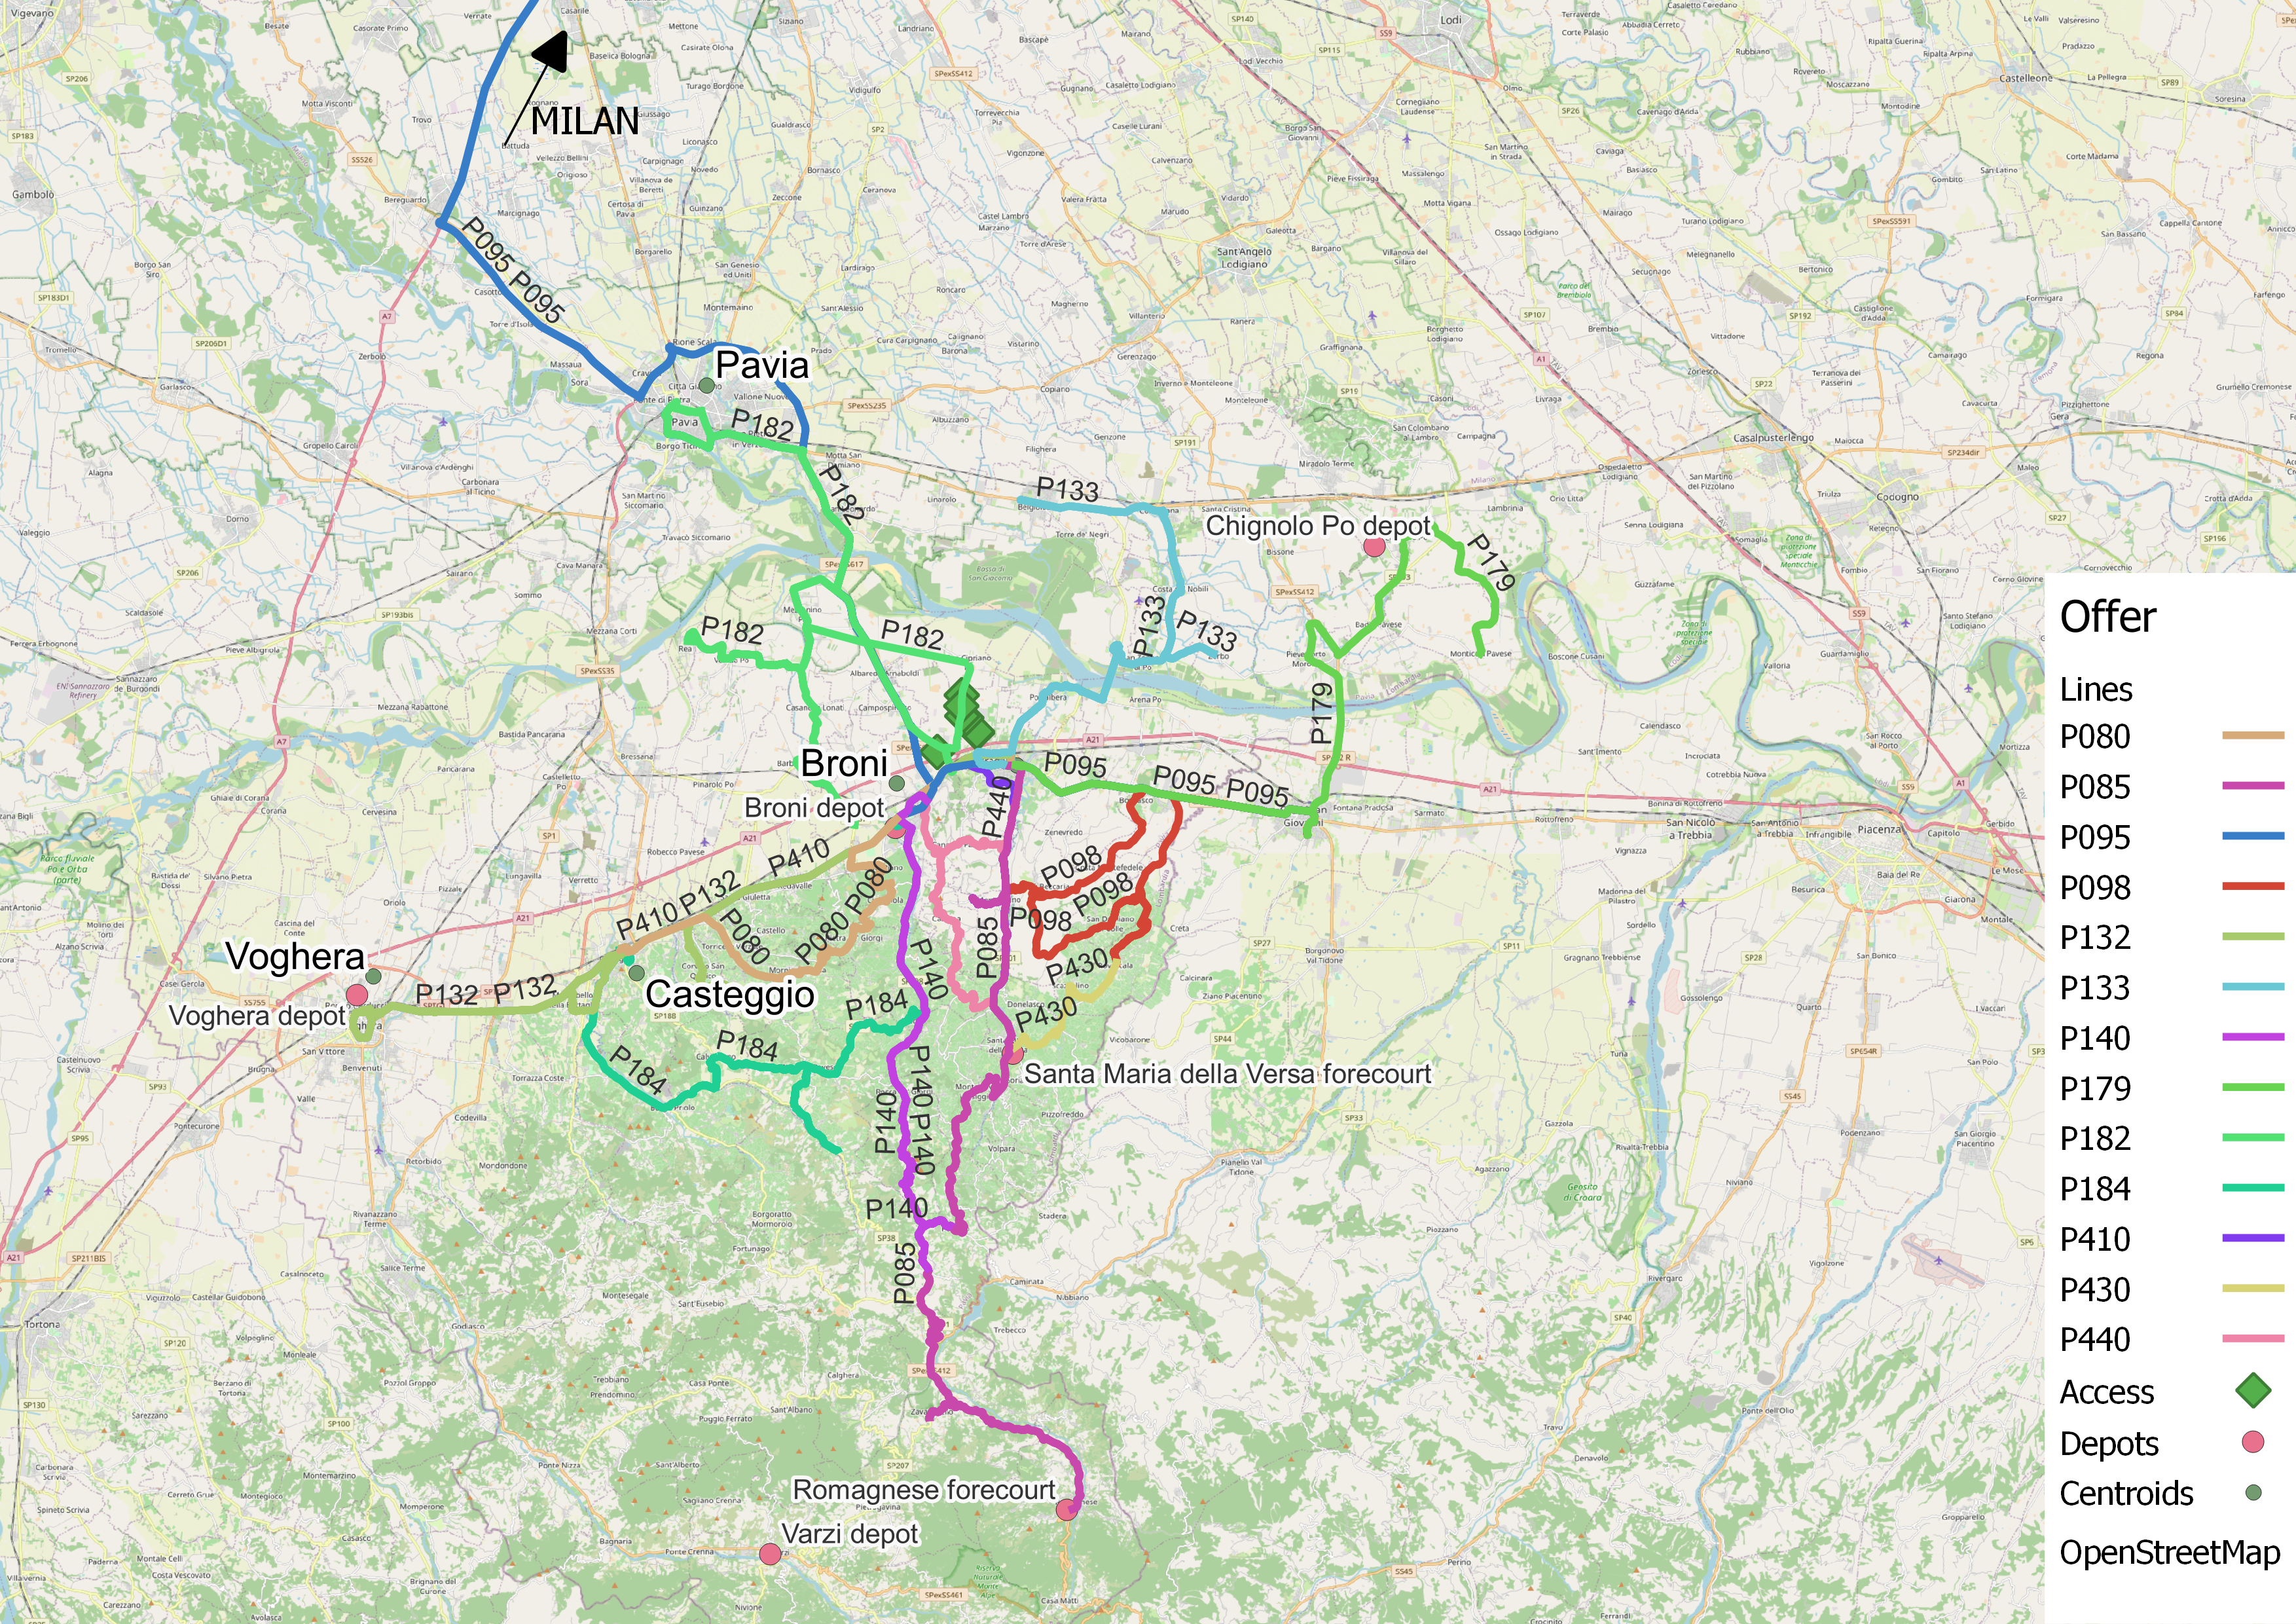
\includegraphics[width=0.7\textwidth]{Images/demand_offer_analysis/Lines.png}
    \caption{The actual offer}
    \label{fig:offer}
\end{figure}

Now in Figure \ref{fig:rail} railway infrastructure from ORM is presented.

\begin{figure}[h]
    \centering
    \includegraphics[width=0.7\textwidth]{Images/demand_offer_analysis/railway.png}
    \caption{The railway infrastructure from ORM}
    \label{fig:rail}
\end{figure}

So, there are railway infrastructure between:

\begin{itemize}
    \item Pavia – Voghera
    \item Voghera- Broni- Stradella - Castel San Giovanni
    \item Pavia – Broni -Stradella – Castel San Giovanni
\end{itemize}
In the analysis of the different timeslots will be also considered the connection with railway service to assess the feasibility of an intermodal approach.

Then with the use of a Python script (algorithm \ref{alg:var}) has been represented the offer in different time slots. It has been considered the departure time from the first stop to be included in the timeslot.

As can be seen in the Figure \ref{fig:offer56} only line P132, P184, P085, P098 have a departure between 05:00 and 06:00.

In Figure \ref{fig:offer730830} Line P095 has two rides that  start between 07:30 and 08:30 \footnote{Note that the result contains all the rides that have a departure between 07:30 and 08:30 but the end time has not been considered. So, a bus can start at 08:25 and it will be considered in the time slot. The analysis would be deepened in the following of the report}.Instead, lines P132, P410, P182, P133, P98, P430 and P095 have only one ride.

In Figure \ref{fig:offer13} the offer increases, because it is the time of exit from school, and a capillary network has been founded with lines P095,P098,P132,P133,P179,P182,P184,P410 and P430 having also a ride that starts in this timeslots.

\begin{figure}
\centering
\subfloat[Lines with departure between 05:00 and 06:00]{\label{fig:offer56}{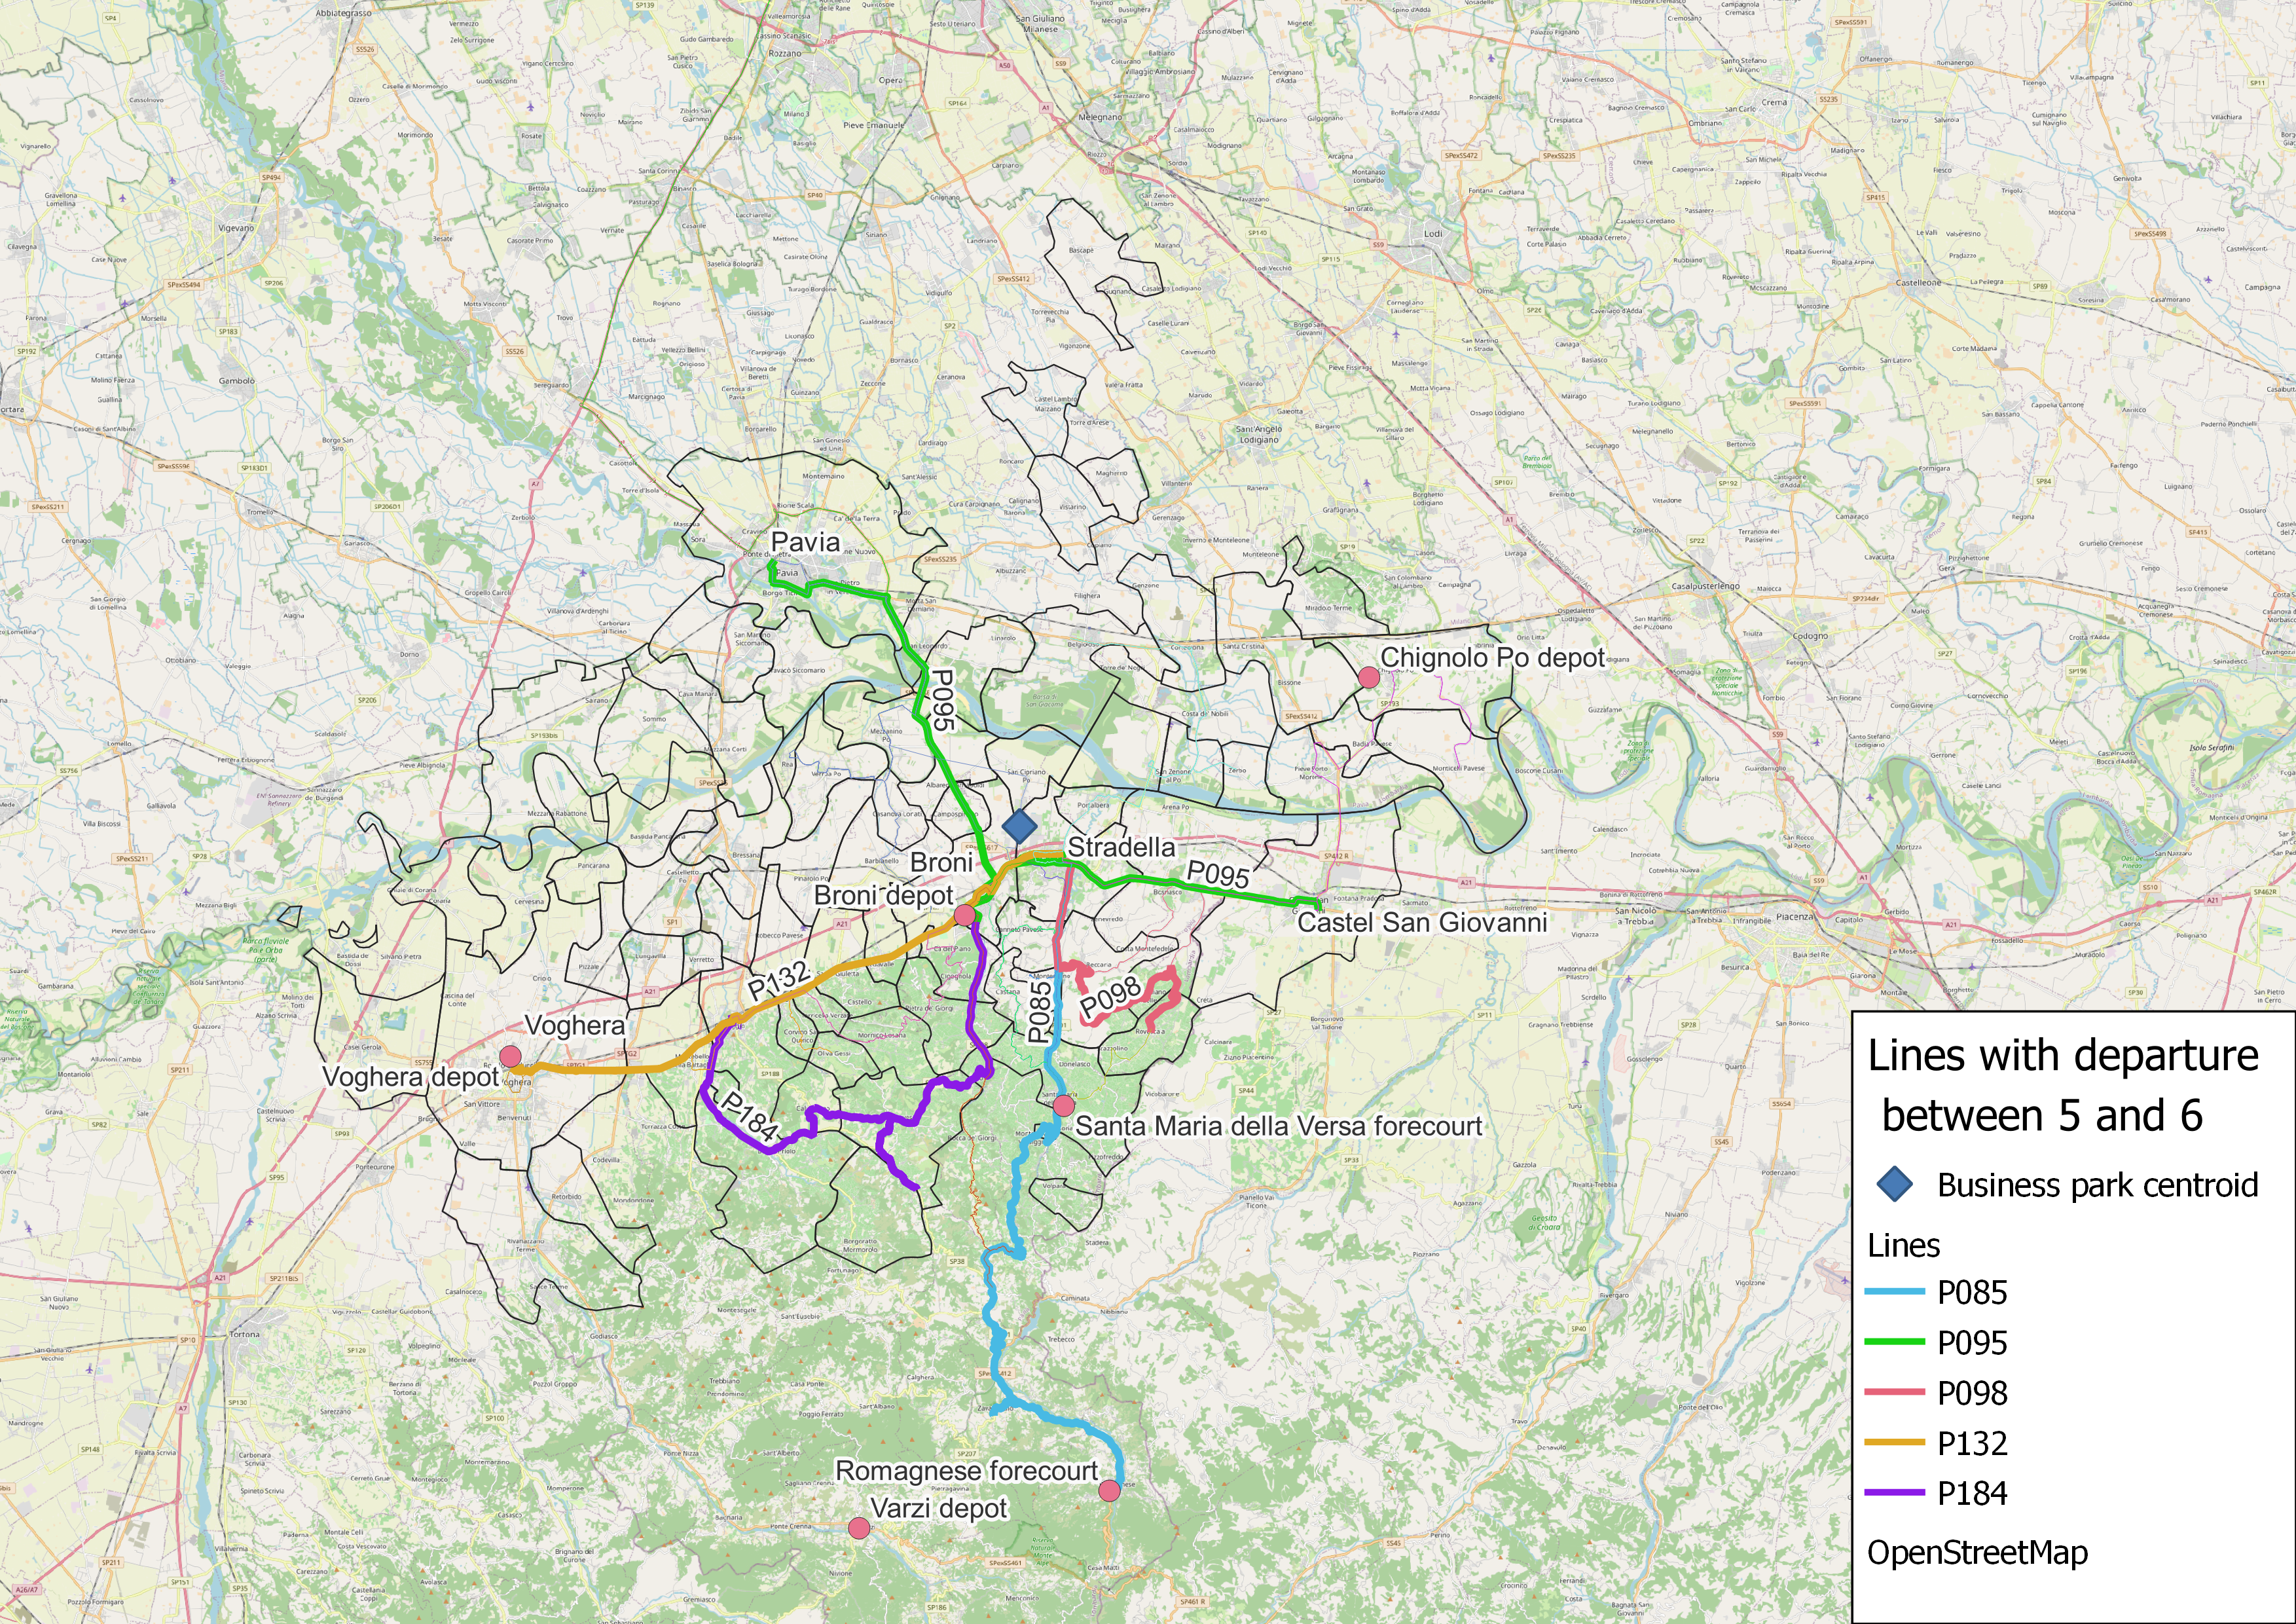
\includegraphics[width=0.6\textwidth]{Images/demand_offer_analysis/Routes_5_6.png}}}\hfill

\subfloat[Lines with departure between 07:30 and 08:30]{\label{fig:offer730830}{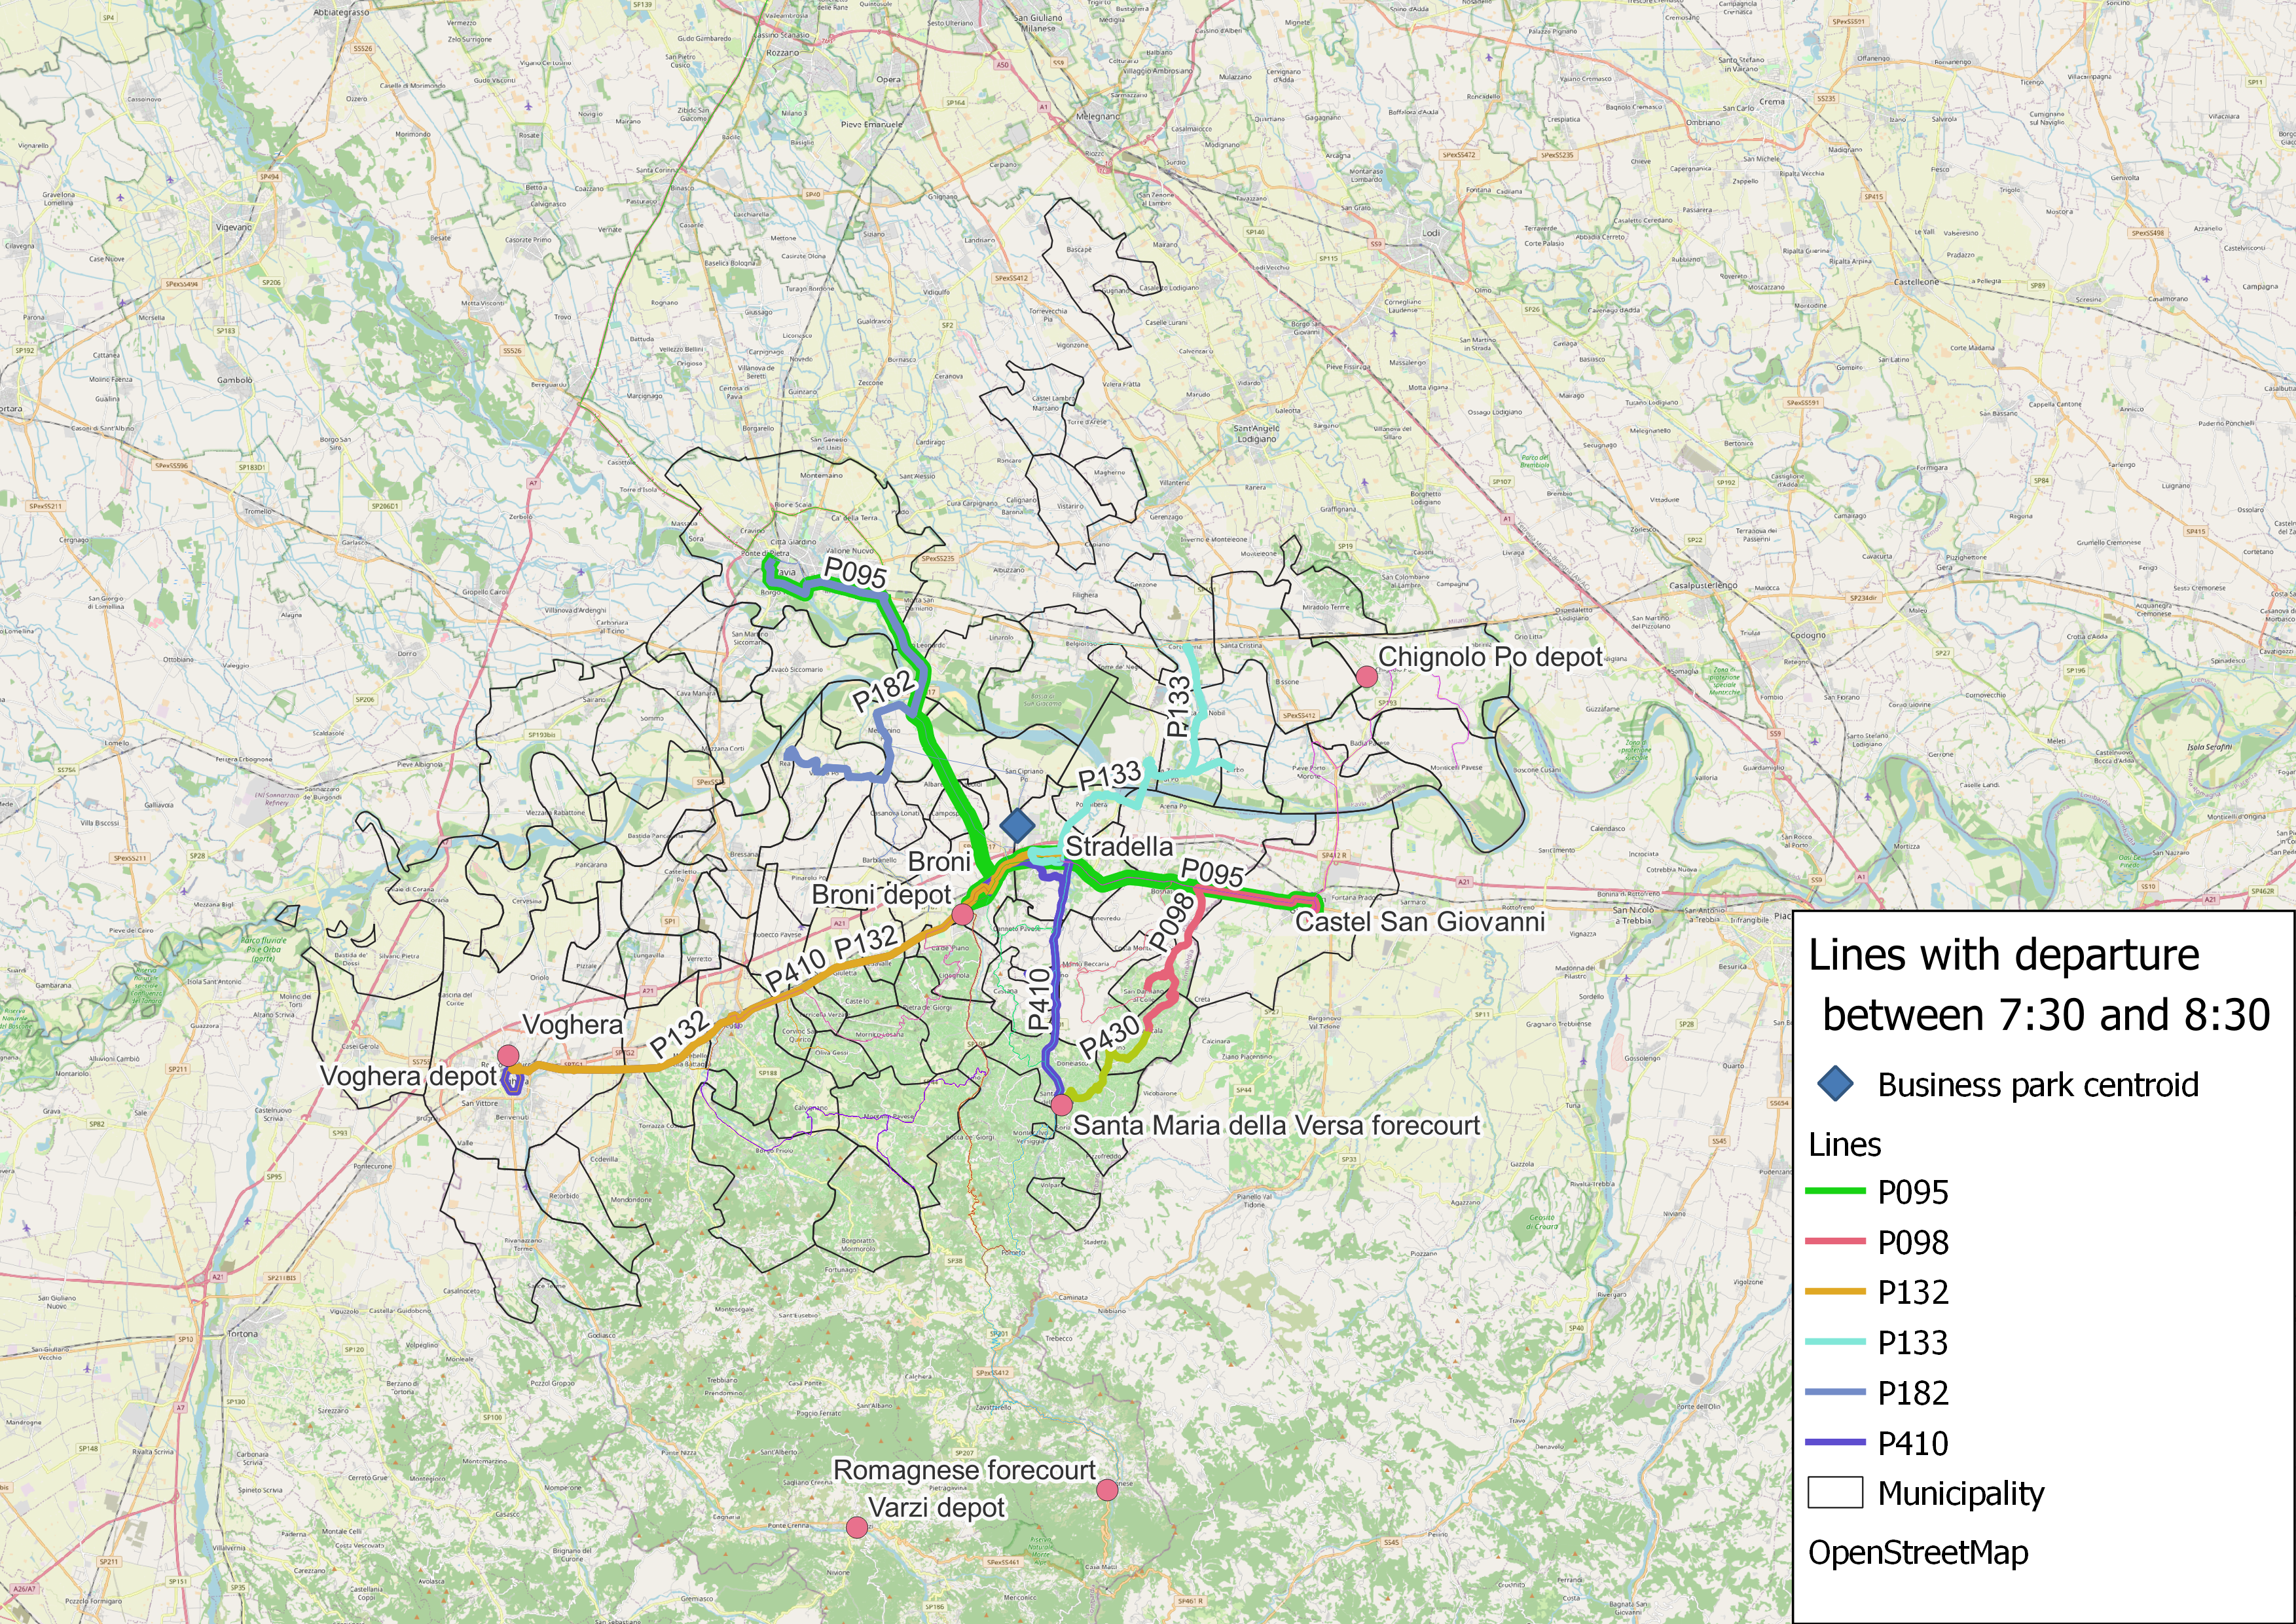
\includegraphics[width=0.6\textwidth]{Images/demand_offer_analysis/730-830.png}}}

\subfloat[Lines with rides that depart between 13 and 14]{\label{fig:offer13}{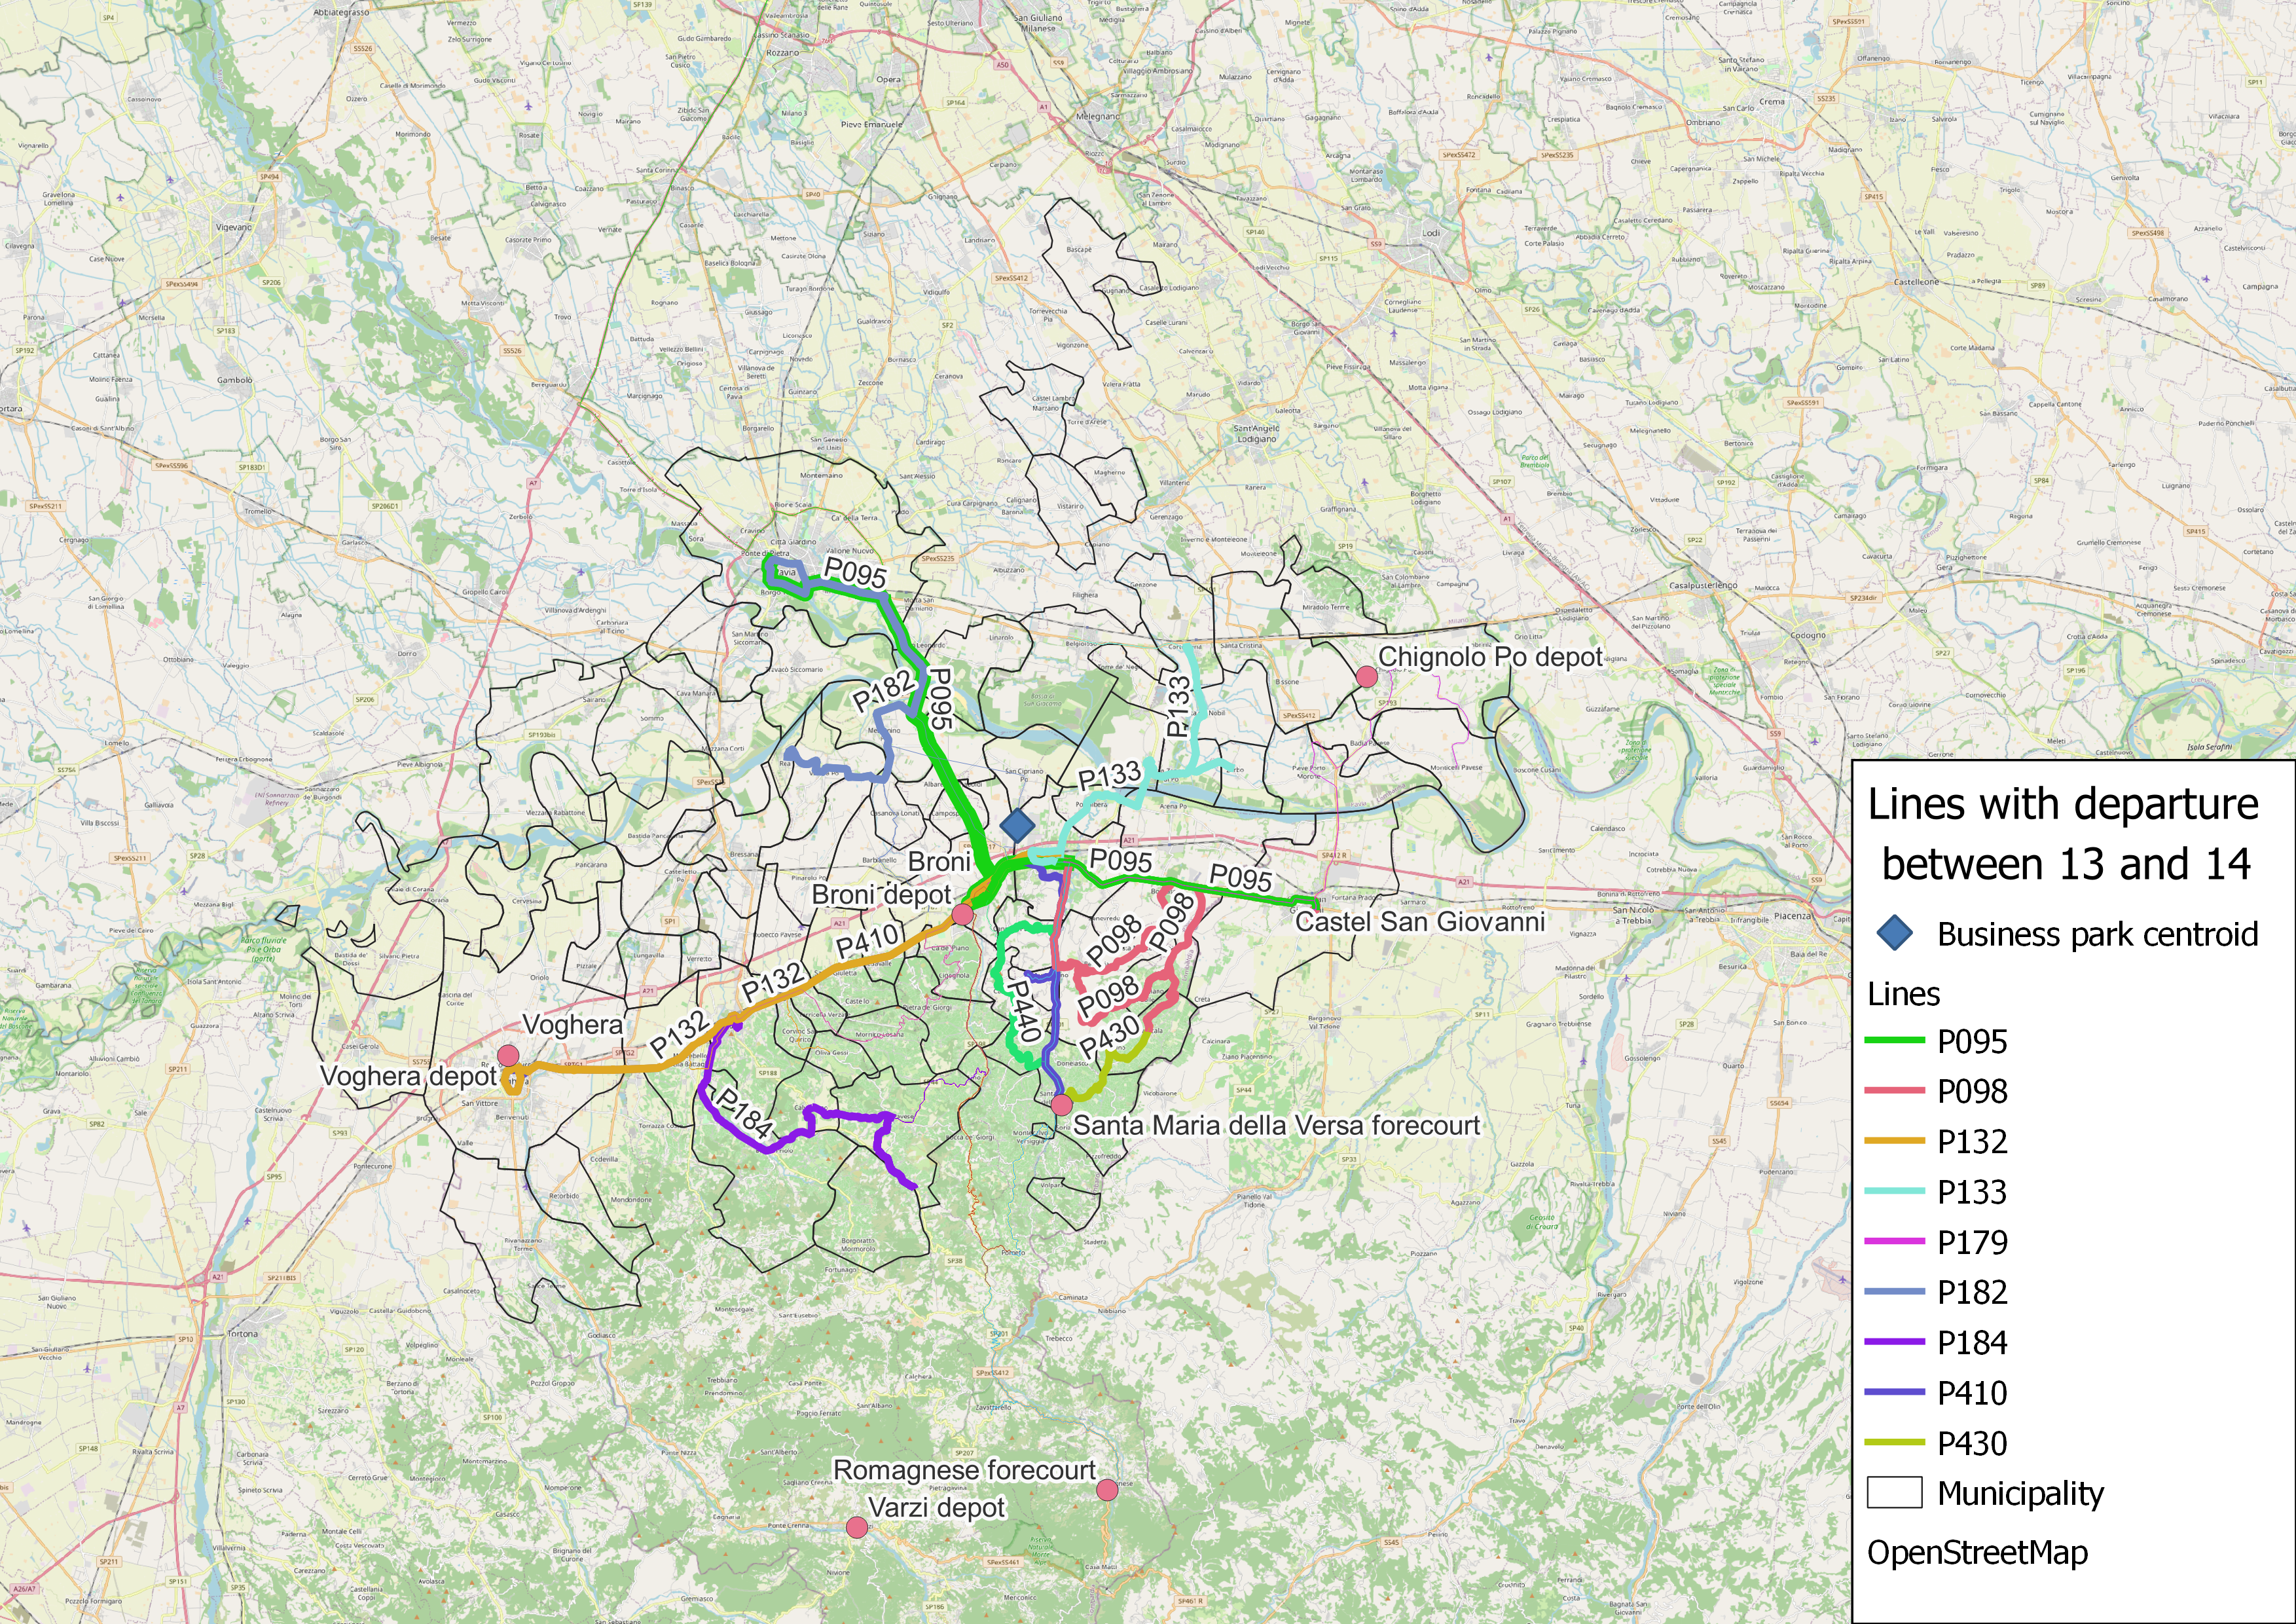
\includegraphics[width=0.6\textwidth]{Images/demand_offer_analysis/13-14.png}}}
\end{figure}

\subsection{Recap on the representation of the offer}
From the analysis it seems that maximum a ride per hour is scheduled. There is no report about the timeslot 21-23 because there are not any rides. For the timeslot 17:30-18:30 the situation is similar to the 07:30-8:30 with the line P95 with higher number of departure.
In addition, after a look to the railway services timetables the intermodal approach is not feasible. This will now argued with an example: considering the shift 06:00-14:00, the train should arrive to Stradella FS at 05:30 to make possible a connection by bus with the Business Park. But looking to the timetables there are not any train rides compatible with that schedule. This makes unfeasible creating an intermodal connection also for the exit time at 14:00, because the workers would arrive at work by bus in the morning, but they would come back with train. This will imply a more complex ticketing system for the users.
 
In other words, an intermodal approach is feasible if can be adopted for entry time and for exit time and for all the shifts. In this case this cannot be applied so in the next sections will be considered only transport by buses.

\section{«Useful» rides and loads}

To evaluate the capacity of the current offer to satisfy the demand it is necessary to identify the useful rides for reaching the business park in each time slot of interest.
In this step of the analysis is not considered yet the demand of mobility in the different areas and the preferences of the customers, that will be included in the next paragraphs.

The useful rides have two characteristics:

\begin{itemize}
    \item Have a compatible route with a terminus or transit near the business park, in order to require only an extension or a deviation of few kilometers
    \item Have a compatible arrival time with the entry time of the workers or require only a slight modification of the timetable
\end{itemize}

The Table \ref{tab:loads} represents the useful rides for each time slot. In the last column of the table is reported also the rides’ loads. The total capacity of the buses is 56 seats due to covid restrictions and some rides’ loads are not available.

For what concern the entry of the worker at 6 in the morning there are not any useful rides, because with an arrival time near the business park too late or too soon, or because they have not a compatible route.

For the entry and the exit of the workers at 22 there are not any rides in those time slots, so not even useful rides.
\newpage
% Please add the following required packages to your document preamble:
% \usepackage[table,xcdraw]{xcolor}
% If you use beamer only pass "xcolor=table" option, i.e. \documentclass[xcolor=table]{beamer}
\newpage
\thispagestyle{empty}
\begin{landscape}
\begin{table}[ht]
\centering
\begin{tabular}{|llllll|}
\hline
\rowcolor{bluepoli!40}
\multicolumn{1}{|c|}{\textbf{Line}} & \multicolumn{1}{c|}{{\color[HTML]{333333} \textbf{Ride code}}} & \multicolumn{1}{c|}{{\color[HTML]{333333} \textbf{Departure   time}}} & \multicolumn{1}{c|}{{\color[HTML]{333333} \textbf{Arrival time}}} & \multicolumn{1}{c|}{{\color[HTML]{333333} \textbf{Route   description}}}  & \multicolumn{1}{c|}{{\color[HTML]{333333} \textbf{Loads}}} \\ \hline
\multicolumn{6}{|c|}{Entry 8.30}                                                                                                                                                                                                                                                                                                                                                          \\ \hline
\multicolumn{1}{|l|}{P095+A2:I3}    & \multicolumn{1}{l|}{195099}                                    & \multicolumn{1}{l|}{07:35}                                            & \multicolumn{1}{l|}{08:06}                                        & \multicolumn{1}{l|}{C.S.GIOV. Gramsci   STRADELLA   BRONI Emilia, 366}    & 8\%                                                        \\ \hline
\multicolumn{1}{|l|}{PV95}          & \multicolumn{1}{l|}{195062}                                    & \multicolumn{1}{l|}{07:40}                                            & \multicolumn{1}{l|}{08:11}                                        & \multicolumn{1}{l|}{C.S.GIOV. Gramsci   STRADELLA   BRONI   Emilia, 366}  & 5\%                                                        \\ \hline
\multicolumn{1}{|l|}{PV95}          & \multicolumn{1}{l|}{195011}                                    & \multicolumn{1}{l|}{07:45}                                            & \multicolumn{1}{l|}{08:35}                                        & \multicolumn{1}{l|}{PV Aut.   P.te Becca   BRONI   STRADELLA Allea}       & 25\%                                                       \\ \hline
\multicolumn{1}{|l|}{PV10010}       & \multicolumn{1}{l|}{410003}                                    & \multicolumn{1}{l|}{07:30}                                            & \multicolumn{1}{l|}{08:02}                                        & \multicolumn{1}{l|}{S.MARIA V.Veneto   STRADELLA   BRONI   Emilia/Italia} & -                                                          \\ \hline
\multicolumn{6}{|c|}{Entry 14}                                                                                                                                                                                                                                                                                                                                                            \\ \hline
\multicolumn{1}{|l|}{PV95}          & \multicolumn{1}{l|}{195025}                                    & \multicolumn{1}{l|}{13:00}                                            & \multicolumn{1}{l|}{13:50}                                        & \multicolumn{1}{l|}{PV Aut.   BRONI   STRADELLA Allea}                    & 45\%                                                       \\ \hline
\multicolumn{1}{|l|}{PV95}          & \multicolumn{1}{l|}{195113}                                    & \multicolumn{1}{l|}{13:09}                                            & \multicolumn{1}{l|}{14:16}                                        & \multicolumn{1}{l|}{C.S.GIOV   STRADELLA   BRONI   PV Aut}                & 75\%                                                       \\ \hline
\multicolumn{1}{|l|}{PV132}         & \multicolumn{1}{l|}{132028}                                    & \multicolumn{1}{l|}{13:10}                                            & \multicolumn{1}{l|}{14:04}                                        & \multicolumn{1}{l|}{VOGHERA   CASTEG FS   BRONI Italia     STRADELLA FS}  & -                                                          \\ \hline
\multicolumn{6}{|c|}{Exit 6}                                                                                                                                                                                                                                                                                                                                                              \\ \hline
\multicolumn{1}{|l|}{PV132}         & \multicolumn{1}{l|}{132003}                                    & \multicolumn{1}{l|}{06:45}                                            & \multicolumn{1}{l|}{07:40}                                        & \multicolumn{1}{l|}{STRAD FS   BRONI Italia   CASTEG FS     VOGHERA}      & 53\%                                                       \\ \hline
\multicolumn{1}{|l|}{PV95}          & \multicolumn{1}{l|}{195153}                                    & \multicolumn{1}{l|}{06:30}                                            & \multicolumn{1}{l|}{07:43}                                        & \multicolumn{1}{l|}{STRAD Battisti   BRONI   P.Becca   MI FAMM2}          & 4\%                                                        \\ \hline
\multicolumn{6}{|c|}{Exit 14}                                                                                                                                                                                                                                                                                                                                                             \\ \hline
\multicolumn{1}{|l|}{PV95}          & \multicolumn{1}{l|}{195031}                                    & \multicolumn{1}{l|}{13:55}                                            & \multicolumn{1}{l|}{14:24}                                        & \multicolumn{1}{l|}{BRONI  C.S.GIOV. Gramsci}                             & 18\%                                                       \\ \hline
\multicolumn{1}{|l|}{PV10040}       & \multicolumn{1}{l|}{440010}                                    & \multicolumn{1}{l|}{13:57}                                            & \multicolumn{1}{l|}{14:45}                                        & \multicolumn{1}{l|}{BRONI   STR V.Ven   CASTAN     S.MARIA V.Ven}         & -                                                          \\ \hline
\multicolumn{1}{|l|}{PV95}          & \multicolumn{1}{l|}{195152}                                    & \multicolumn{1}{l|}{14:00}                                            & \multicolumn{1}{l|}{15:04}                                        & \multicolumn{1}{l|}{PV Aut.   BRONI   STRAD     C.S.GIOV Gramsci}         & 49\%                                                       \\ \hline
\multicolumn{1}{|l|}{PV10010}       & \multicolumn{1}{l|}{410027}                                    & \multicolumn{1}{l|}{14:09}                                            & \multicolumn{1}{l|}{14:40}                                        & \multicolumn{1}{l|}{BRONI   STRADELLA   S.MARIA V.Veneto}                 & -                                                          \\ \hline
\multicolumn{1}{|l|}{PV80}          & \multicolumn{1}{l|}{80032}                                     & \multicolumn{1}{l|}{14:10}                                            & \multicolumn{1}{l|}{15:02}                                        & \multicolumn{1}{l|}{STRA Batt BRO Italia . CASTEGGIO FS}                  & -                                                          \\ \hline
\multicolumn{1}{|l|}{PV132}         & \multicolumn{1}{l|}{132031}                                    & \multicolumn{1}{l|}{14:15}                                            & \multicolumn{1}{l|}{15:03}                                        & \multicolumn{1}{l|}{STRADELLA FS   BRONI Italia   VOGHERA   Aut.}         & 52\%                                                       \\ \hline
\multicolumn{1}{|l|}{PV95}          & \multicolumn{1}{l|}{195119}                                    & \multicolumn{1}{l|}{14:40}                                            & \multicolumn{1}{l|}{15:27}                                        & \multicolumn{1}{l|}{STRADELLA Trieste   BRONI   P.te Becca   PAV Aut.}    & 18\%                                                       \\ \hline
\multicolumn{1}{|l|}{PV10010}       & \multicolumn{1}{l|}{410022}                                    & \multicolumn{1}{l|}{14:45}                                            & \multicolumn{1}{l|}{15:20}                                        & \multicolumn{1}{l|}{BRONI Ita   STR V.Ven   S.MARIA V.Veneto}             & -                                                          \\ \hline
\multicolumn{6}{|c|}{Exit 17.30}                                                                                                                                                                                                                                                                                                                                                          \\ \hline
\multicolumn{1}{|l|}{PV184}         & \multicolumn{1}{l|}{184033}                                    & \multicolumn{1}{l|}{17:50}                                            & \multicolumn{1}{l|}{19:05}                                        & \multicolumn{1}{l|}{STRADELLA Battisti   CALV B.PRI   CASTEGGIO}          & -                                                          \\ \hline
\multicolumn{1}{|l|}{PV85}          & \multicolumn{1}{l|}{85020}                                     & \multicolumn{1}{l|}{17:55}                                            & \multicolumn{1}{l|}{19:18}                                        & \multicolumn{1}{l|}{STRAD V.Ven   S.MARIA V   ROMAGNESE Pesa}             & -                                                          \\ \hline
\end{tabular}
\caption{Useful rides}
\label{tab:loads}
\end{table}
\end{landscape}
\newpage
\newpage
\section{Demand}

The analysis is based on an Excel file that contains two worksheets about the weighted number of the shifts\footnote{he workers change the shifts by days, so the demand is weighted to have a real estimation of the demand. The daytime is not weighted because is fix.}  and the preferences of means of transport.
There are four work shifts:

\begin{itemize}
    \item 06:00-14:00
    \item 14:00-22:00
    \item 22:00-06:00
    \item 08:30-17:30
\end{itemize}
So given the provided data and the shapefile \cite{Istat2022CONFINI2022} the demand has been plotted.

\paragraph{Demand shift 06:00 - 14:00}

Figure \ref{fig:demand614} represents the desired lines based on the demand.

The municipalities in the zone with the lowest demand are not considered because their demand is too low and with high preference for private car.

Stradella and Broni represent the municipalities with highest demand. They are also the ones with lowest willingness to use the public transport. This because they are the nearest to the Business Park. Nevertheless, the number of people that will use the public transport justifies taking them in consideration. 

Following a similar reasoning also Voghera should be considered.

Surprisingly Pavia has the same level of demand of Casteggio and Castel San Giovanni. Those municipality whose demand is the second lowest should be considered only if this do not require important changes of the services.

\paragraph{Demand shift 14:00 - 22:00}
Pavia, Casteggio and Castel San Giovanni remain with the same level of demand and for this reason will be considered only if the changes will not impact too much the services.
So, we consider only Stradella, Broni and Voghera. 

\paragraph{Demand shift  22:00 - 6:00}
In the timeslot, represented by Figure \ref{fig:demand226}, it is evident a reduction of the demand. The only municipalities considerable are Stradella, Broni and Voghera.


\paragraph{Demand shift 08:30 - 17:30}
Also in this case, the municipalities with the highest demand are Broni and Stradella. As before the municipalities in the second zone will be considered only if the changes should not be too important.

\begin{figure}
\centering
\subfloat[Demand and desired lines for shift 06:00 - 14:00]{\label{fig:demand614}{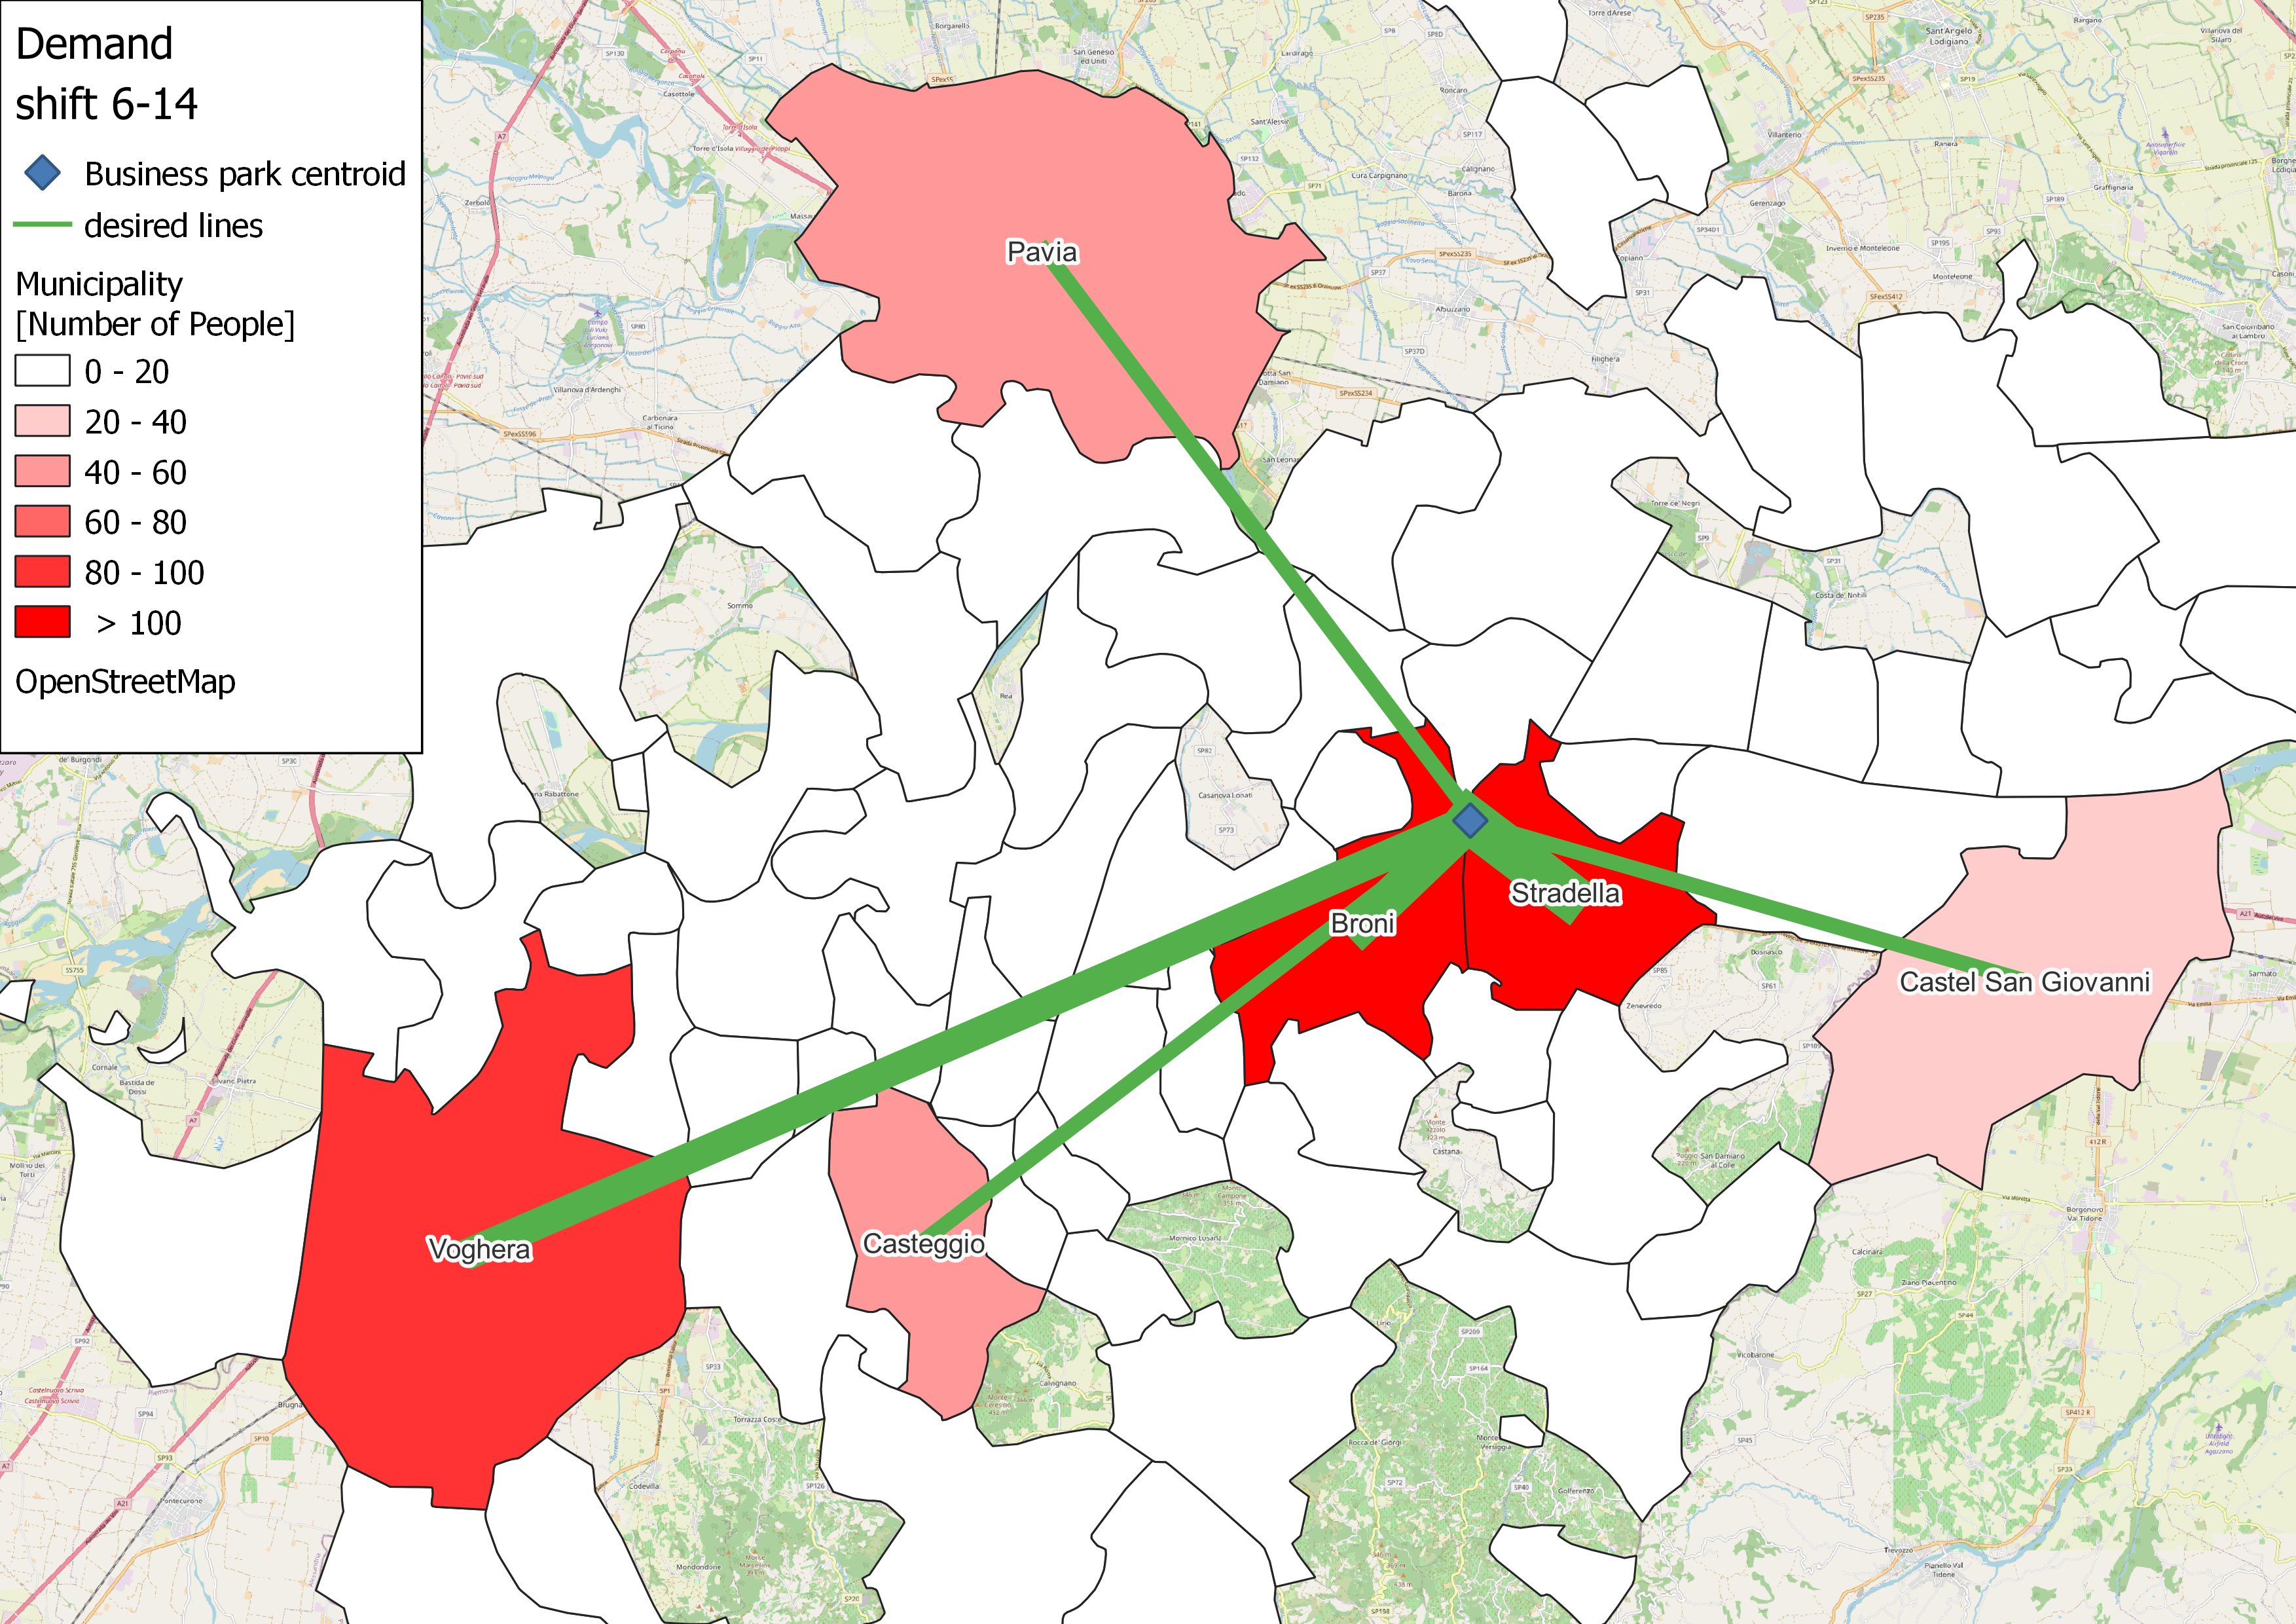
\includegraphics[width=0.8\textwidth]{Images/demand_offer_analysis/desired_lines_6-14.png}}}\hfill
\subfloat[Demand and desired lines for shift  14:00 22:00]{\label{fig:demand1422}{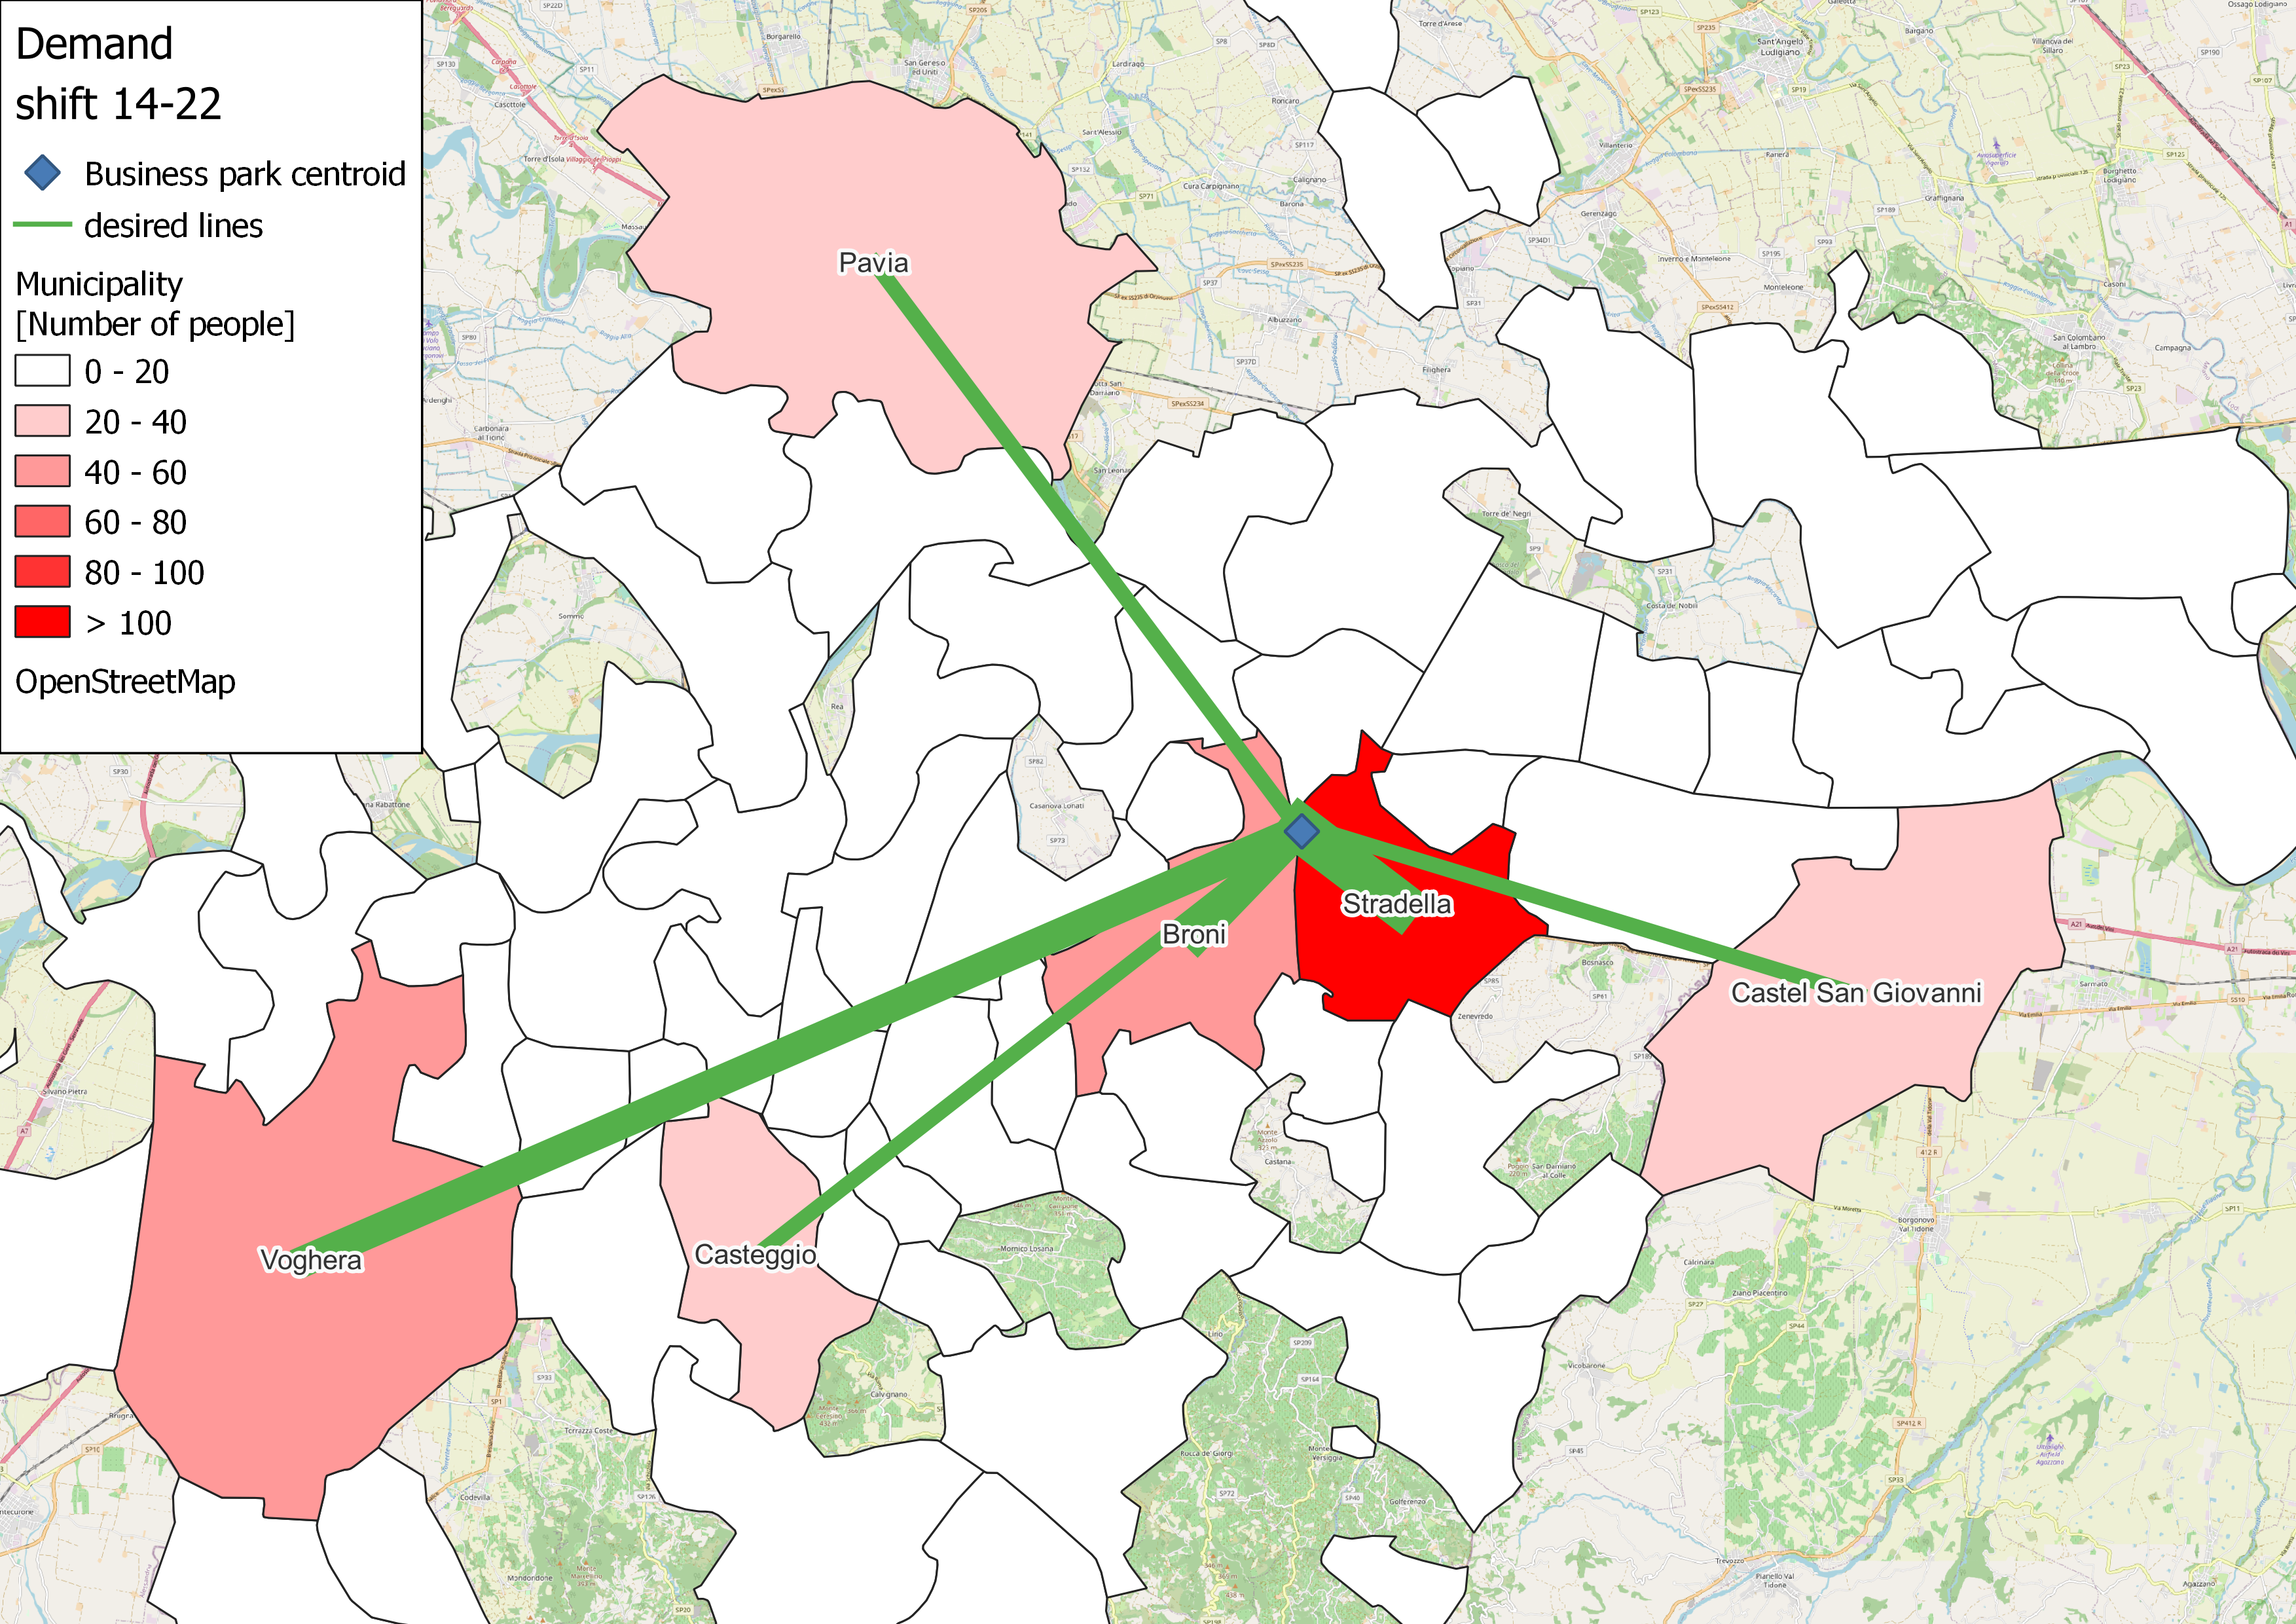
\includegraphics[width=0.8\textwidth]{Images/demand_offer_analysis/desired_lines_14-22.png}}}
\end{figure}

\begin{figure}
    \centering
\subfloat[Demand and desired lines for shift 22:00 06:00]{\label{fig:demand226}{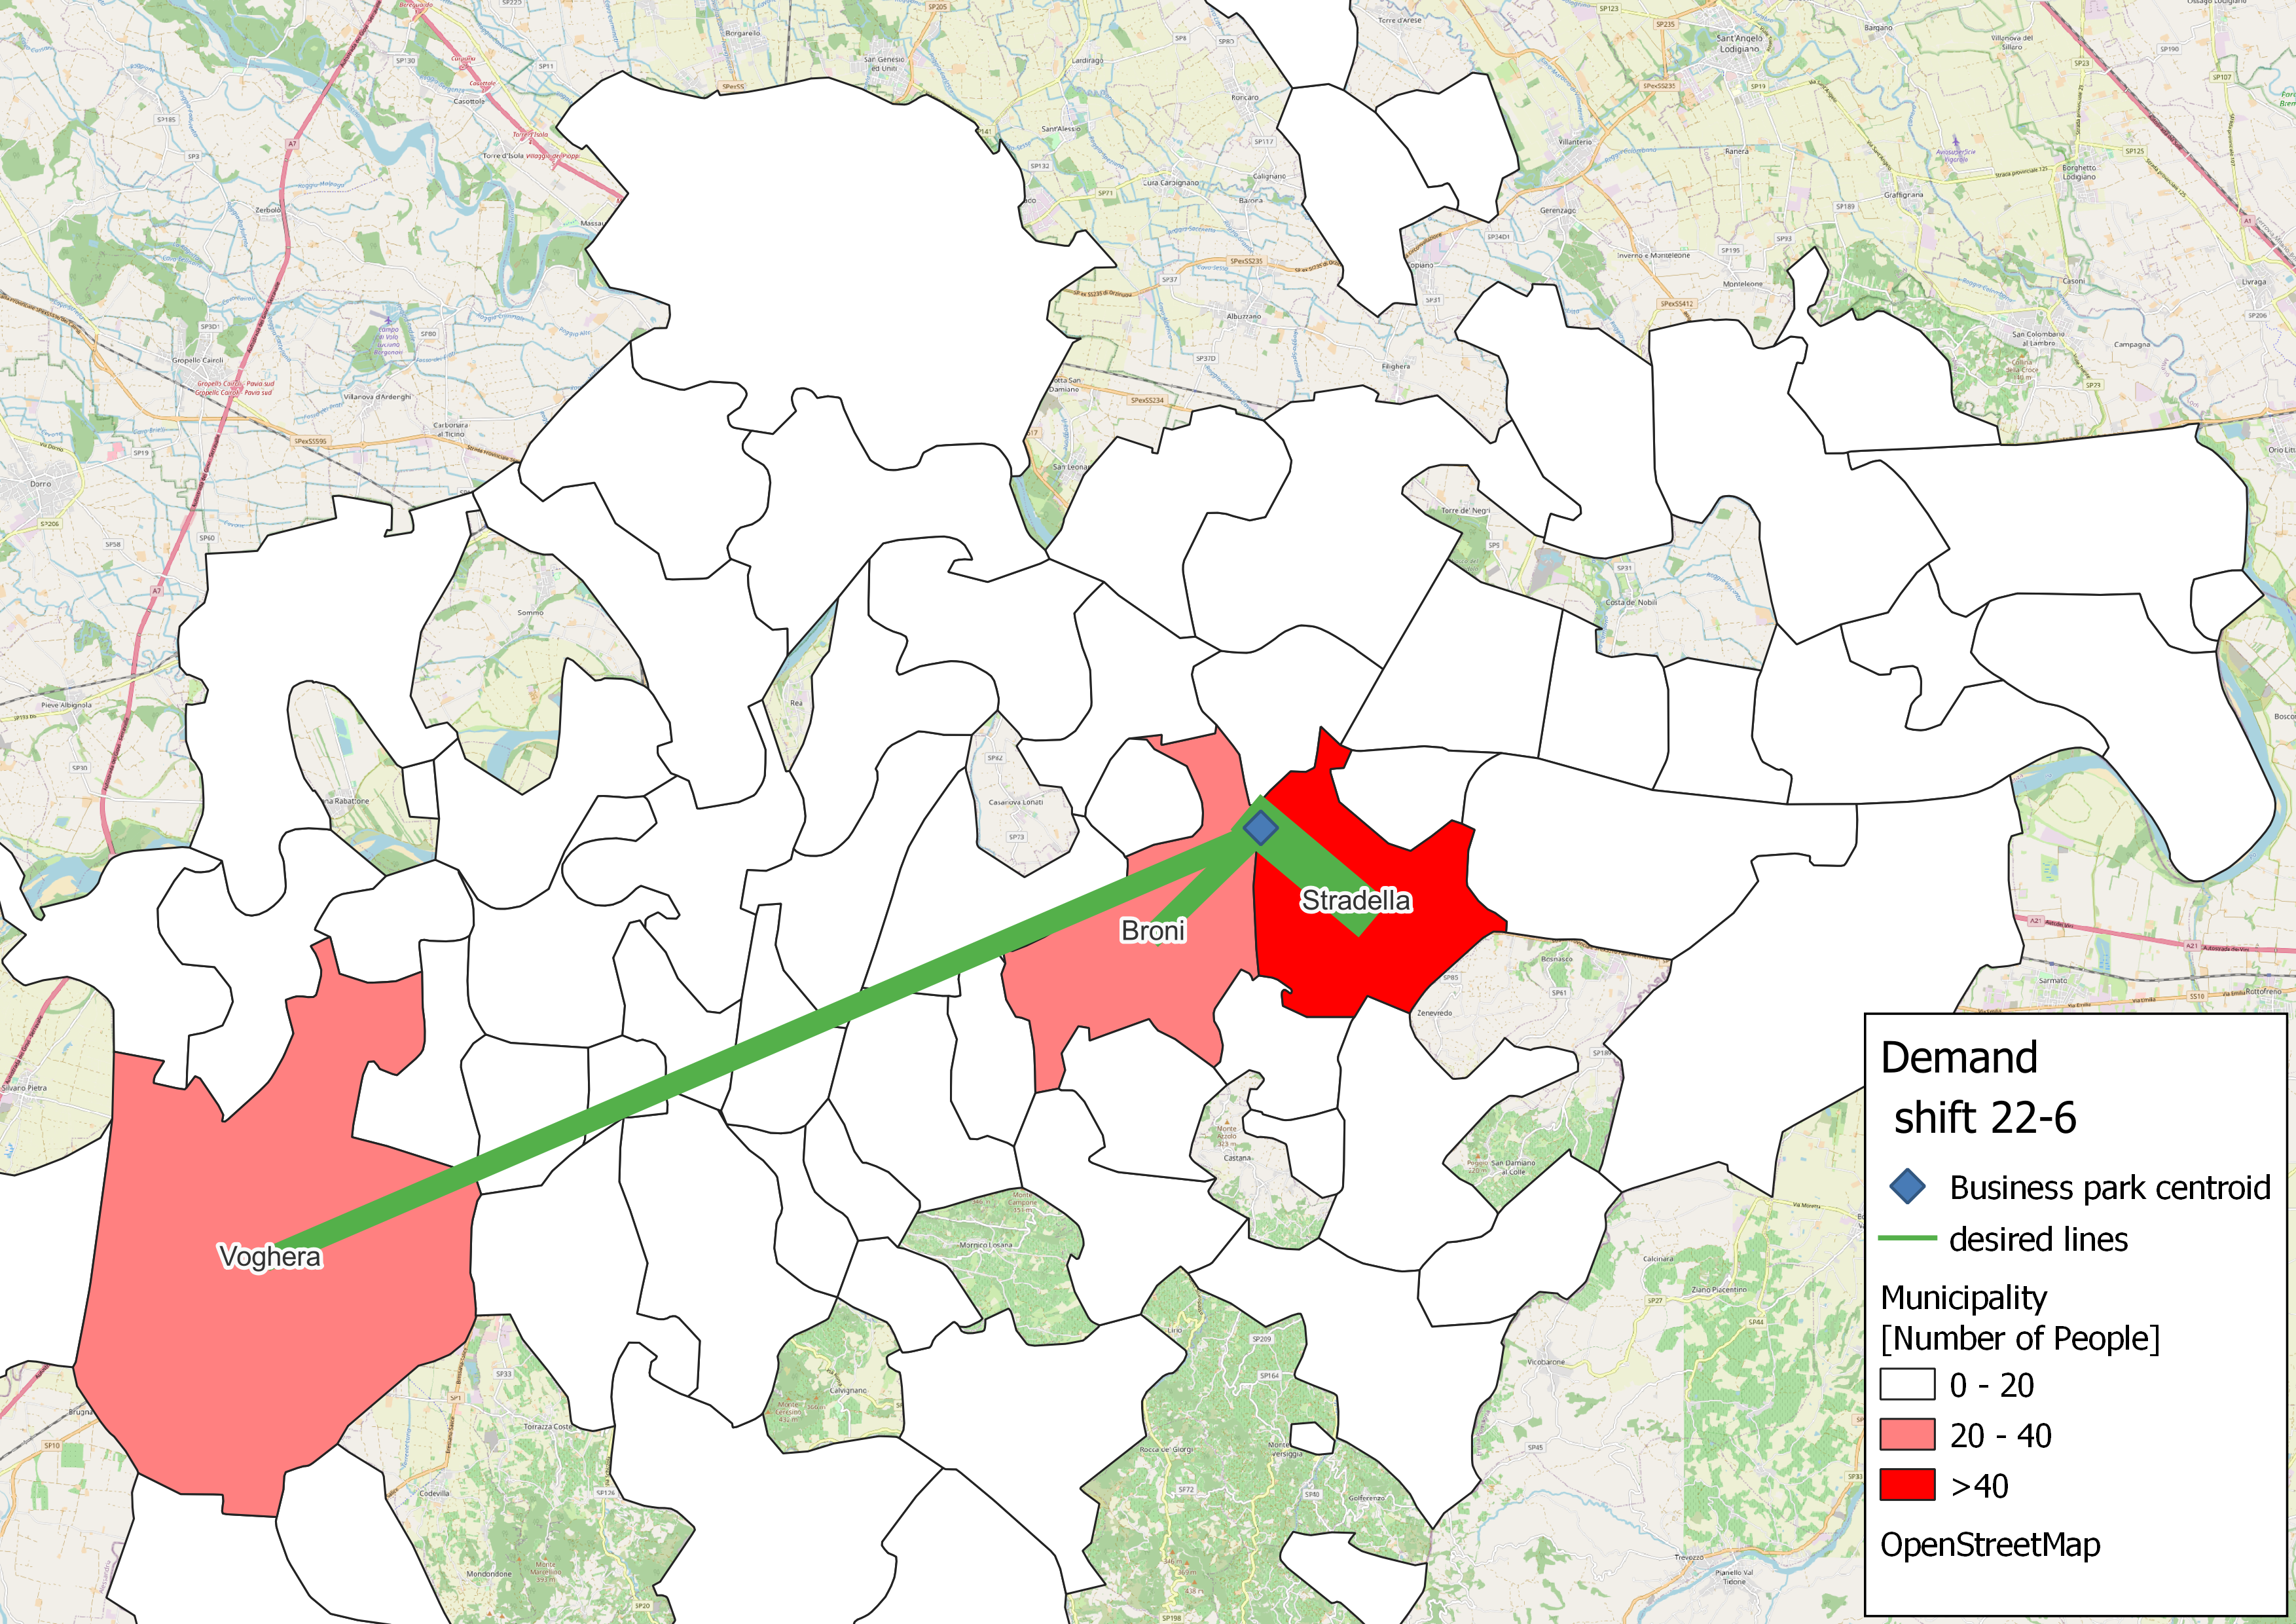
\includegraphics[width=0.8\textwidth]{Images/demand_offer_analysis/desirered_lines_22_6.png}}}\hfill
\subfloat[Demand and desired lines for daytime]{\label{fig:demand8301730}{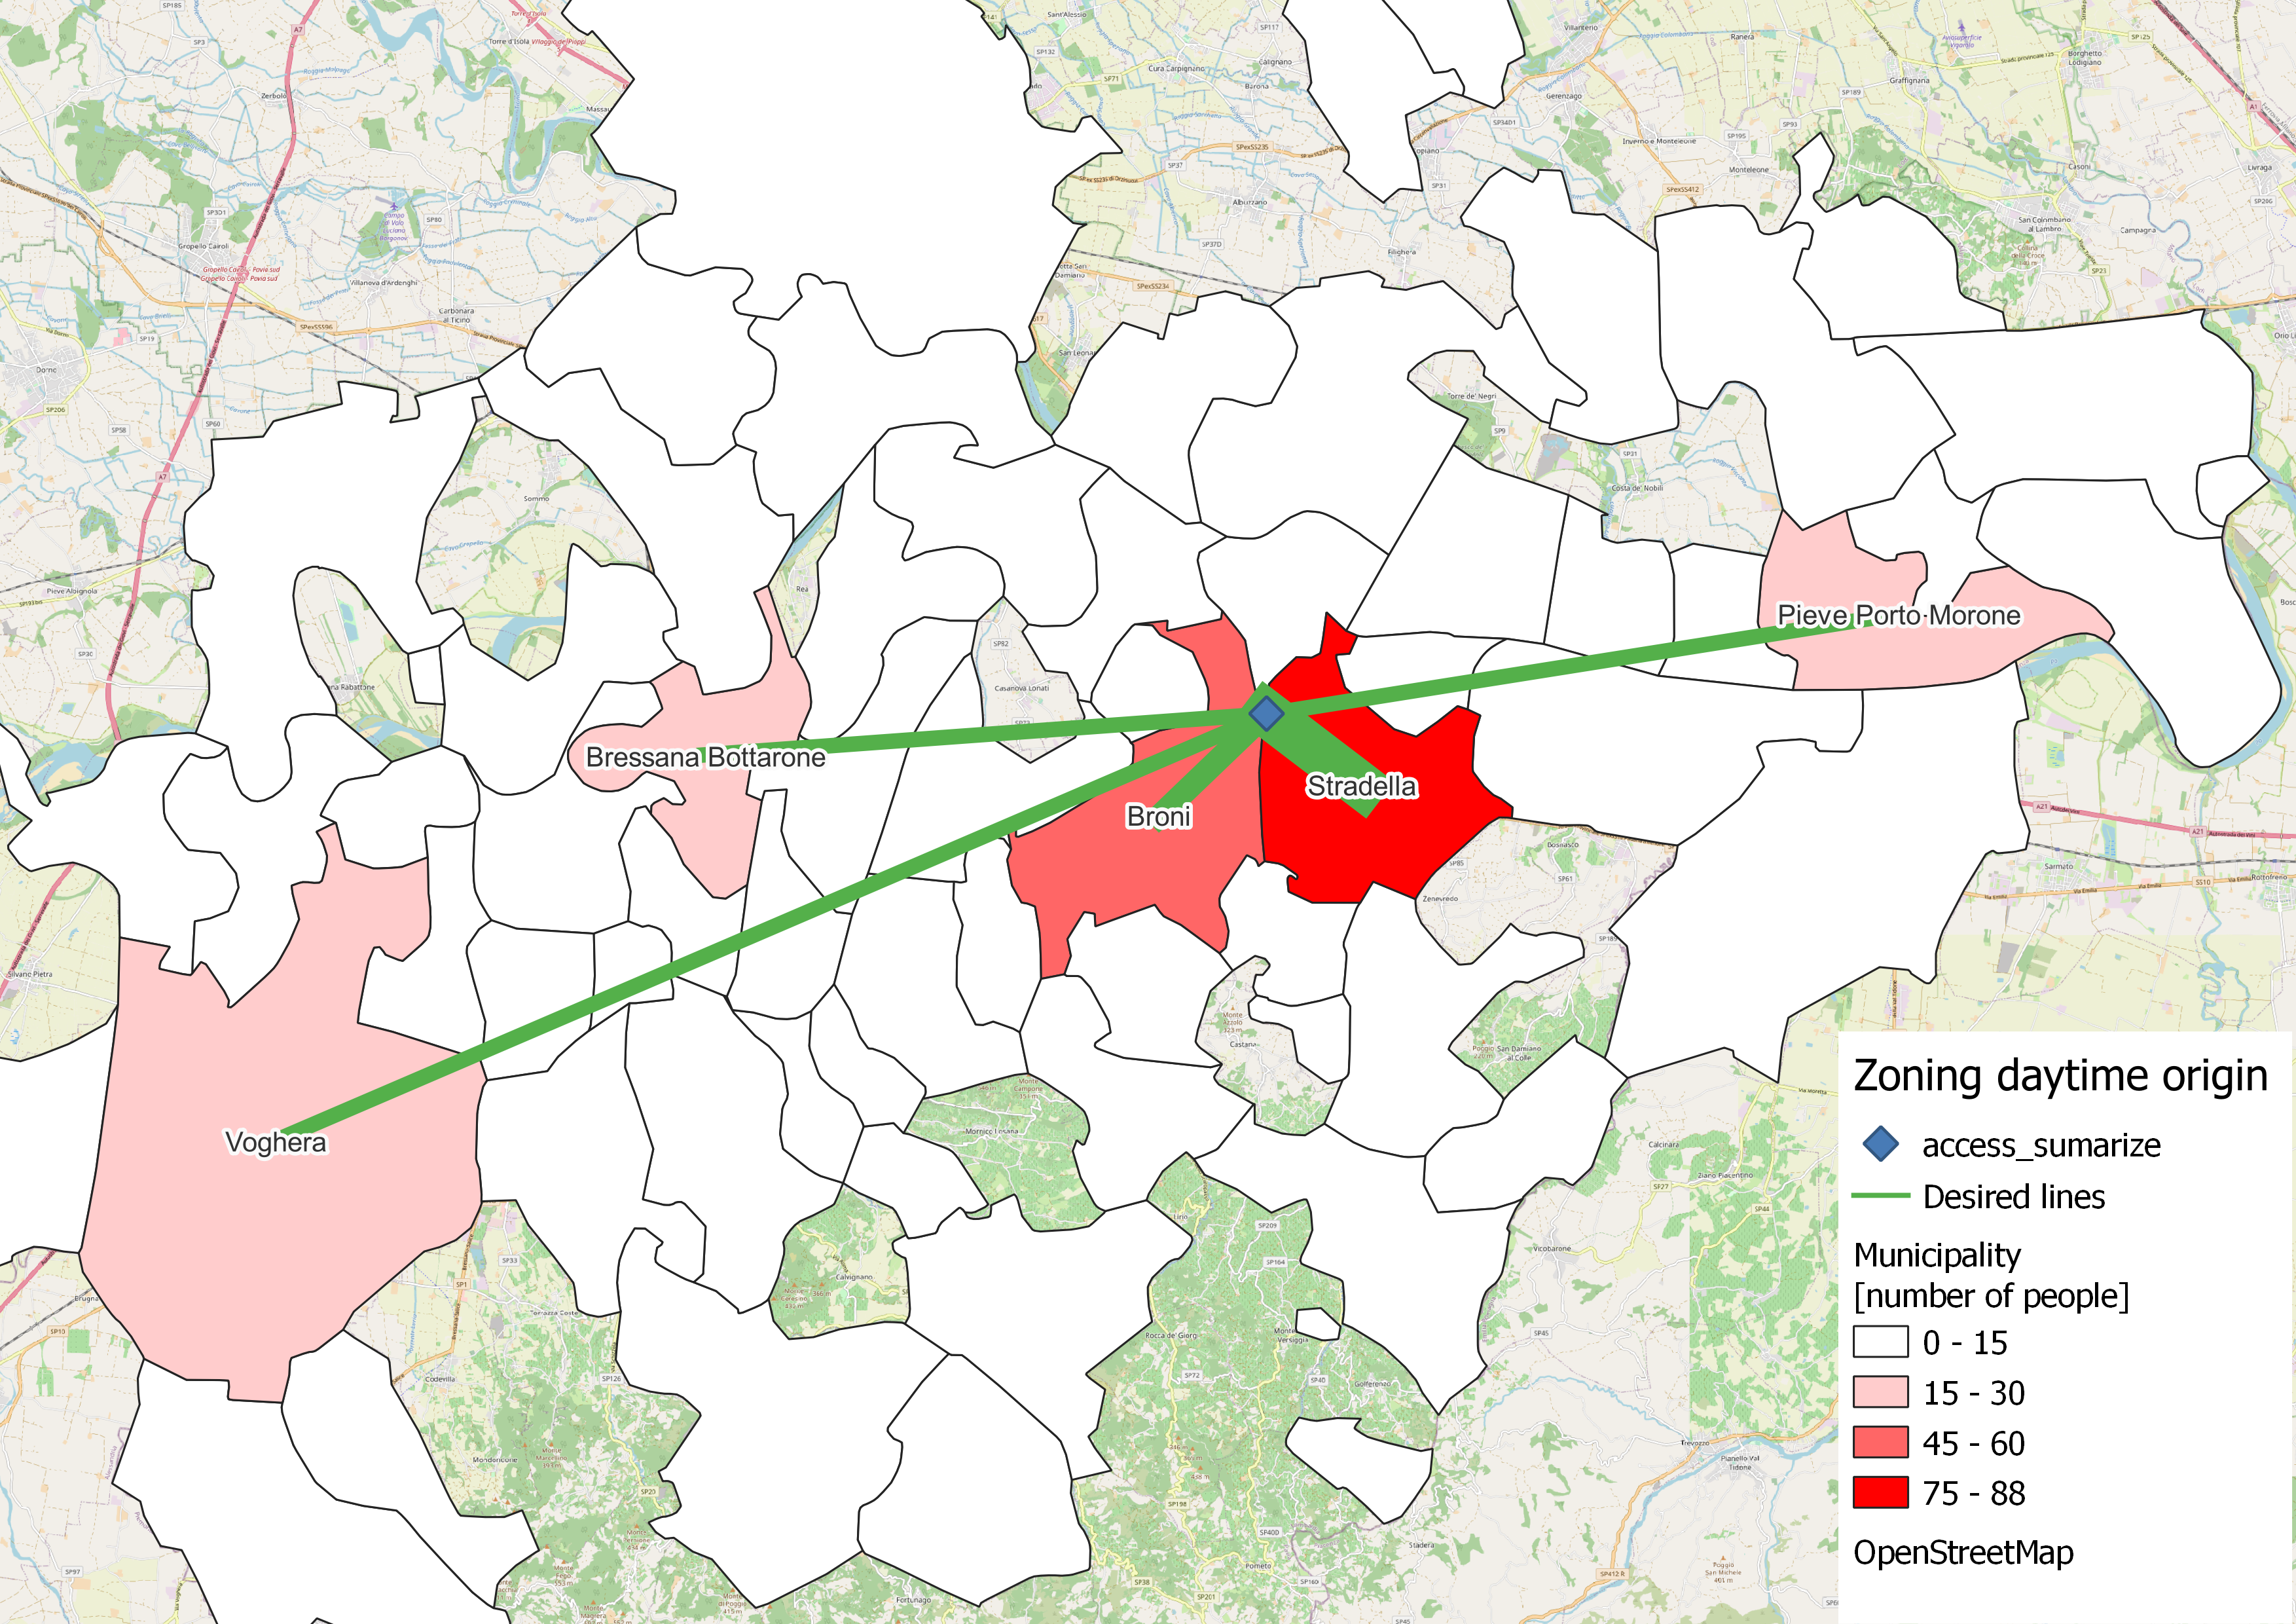
\includegraphics[width=0.8\textwidth]{Images/demand_offer_analysis/desired lines daytime.png}}}
\end{figure}

\paragraph{Means of transport preference}
Means of transport preference shown in Figure 10 does not depend on the shift, but they are general. 

\begin{figure}[h]
    \centering
    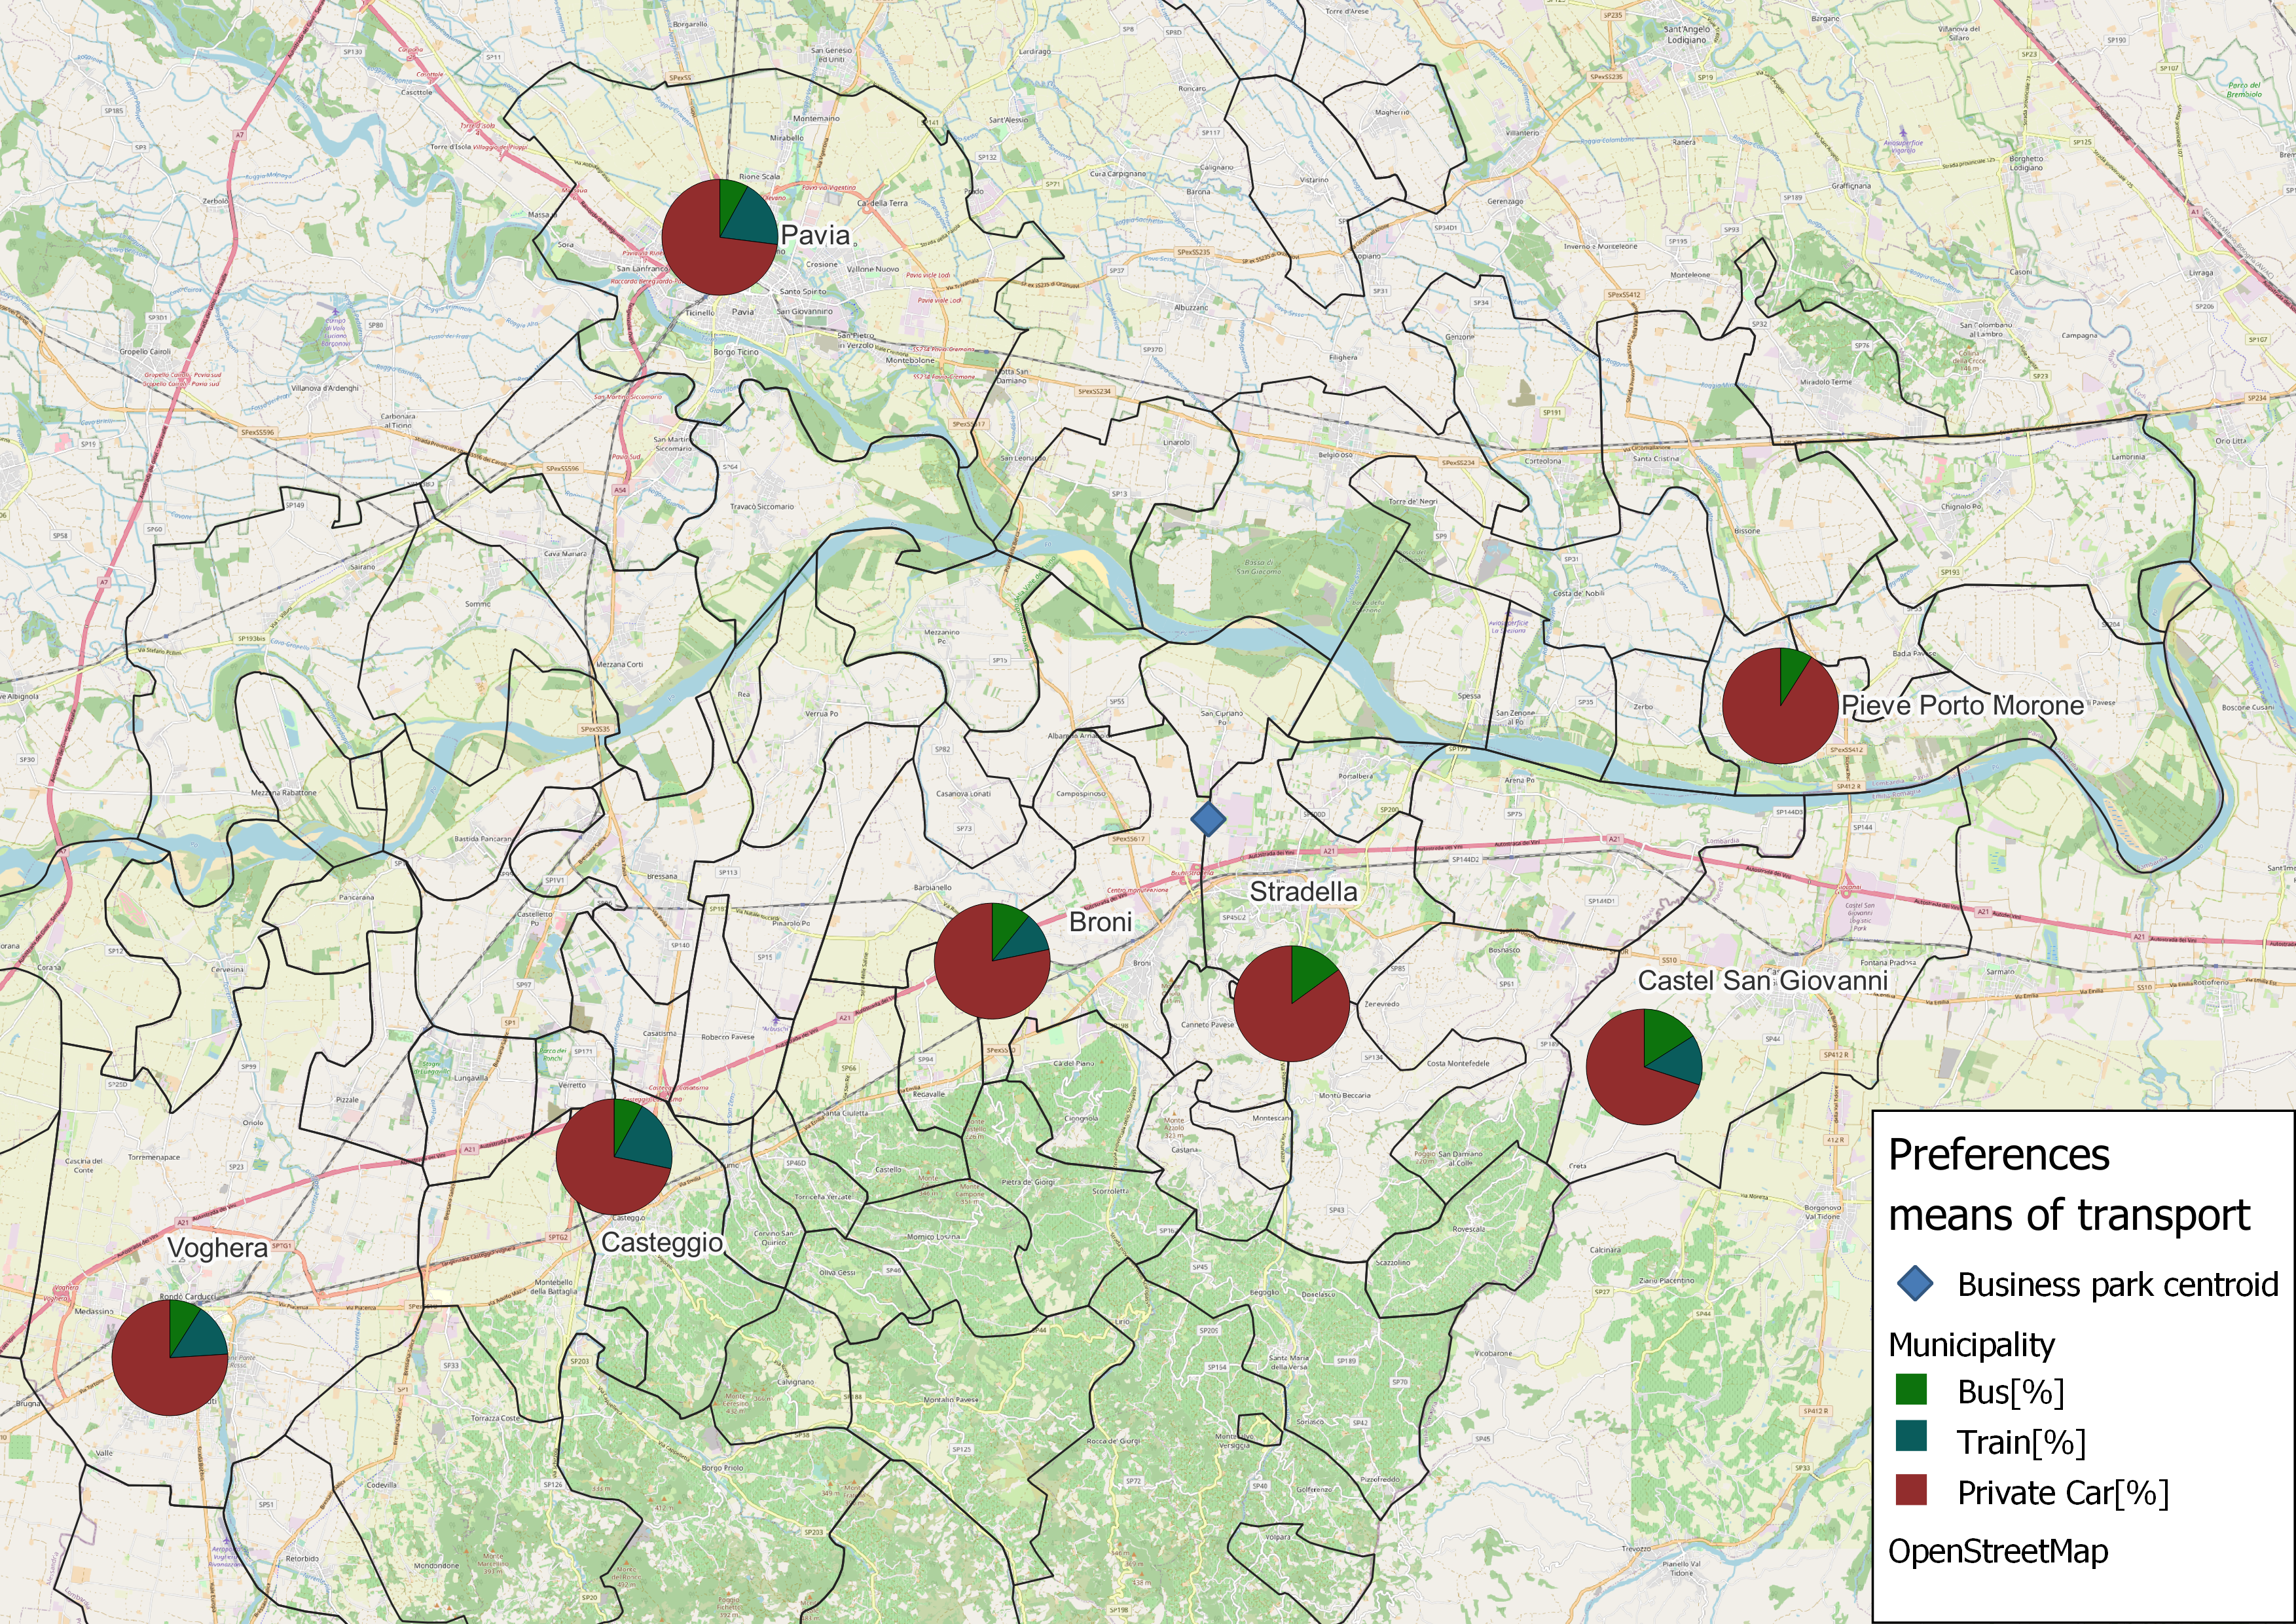
\includegraphics[width=0.7\textwidth]{Images/demand_offer_analysis/preferences.png}
    \caption{The preferences for the means of transport}
    \label{fig:meantransport}
\end{figure}

The plot shows an average value of 20\% of people that will choose a public transport  with a peak of preference for the train in the municipalities that have a railway station.
Broni and Stradella has the lowest preference for public transport. This is probably due to the fact that they are also the nearest to the business park.
In Table \ref{tab:transportcount} there is an estimation, based on the provided data, about the number of people that will use the public transport. This will return useful in \ref{ch:sizeschedule}
\newpage
% Please add the following required packages to your document preamble:
% \usepackage{lscape}
%\begin{landscape}
\begin{table}[h]
\centering
\begin{tabular}{|l|l|l|l|l|}
\hline
\rowcolor{bluepoli!40}
\multicolumn{1}{|c|}{\textbf{Municipality}} & \multicolumn{1}{c|}{\textbf{06:00-14:00}} & \multicolumn{1}{c|}{\textbf{14:00-22:00}} & \multicolumn{1}{c|}{\textbf{22:00-6:00}} & \multicolumn{1}{c|}{\textbf{08:30-17:30}} \\ \hline
Voghera                                     & 19                                        & 14                                        & 5                                        & 5                                         \\ \hline
Stradella                                   & 22                                        & 17                                        & 8                                        & 13                                        \\ \hline
Broni                                       & 25                                        & 13                                        & 6                                        & 10                                        \\ \hline
Casteggio                                   & 13                                        & 8                                         & 3                                        & 4                                         \\ \hline
Castel San Giovanni                         & 8                                         & 7                                         & 2                                        & 2                                         \\ \hline
Pieve   Porto morone                        & 1                                         & 0                                         & 0                                        & 1                                         \\ \hline
\end{tabular}
\caption{Number of people that will use public transport}
\label{tab:transportcount}
\end{table}
%\end{landscape}
\newpage

\section{Match offer and demand}

The last step of the first part of the project is the comparison between the current offer and the desired lines identified previously. In this way it is possible to see if there are existing rides which can satisfy the demand with small changes or without changes. For the time slots and for the desired routes that are not covered by the current service it is necessary to identify some proposals to satisfy the demand.
The elements considered in the identification of the proposals are:
\begin{itemize}
    \item Workers should be brought as close as possible to the accesses of the business park, so there will be the need to identify new stops near the Business Park
    \item Workers must arrive at the entrance of the Business Park at least ten minutes before the start of the shift to ensure that they can respect working hours. Even for the end of the shift, at least 10 minutes are considered to reach the bus stops.
    \item The possibility to have an intermodal service with an interchange at Stradella FS and a shuttle has been considered, but this option is not suitable because in the hours of our interest there are not any train from and to the municipalities of our interest.
\end{itemize}

\paragraph{06:00 - 14:00}

\subparagraph{Entry 6:00} In this time slot there are not any useful rides that can satisfy the demand, as previously said in the paragraph 1.2. As we can notice from the Figure 6 the municipalities with the highest demand are Voghera, Broni and Stradella. For the satisfaction of this demand, we suggest a new ride of the line PV132, with the route code P13201 and an extension of the ride from Stradella FS to the Business Park. The additional stops will be defined in the paragraph 2.1.The ride must arrive before the 5:50 to ensure the workers to respect working hours.

For the municipalities with lower demand, such as Pavia and Castel San Giovanni, we suggest to not add a ride or a line because the changes to be made to the timetable are considerable and not justified by a very low demand.

\subparagraph{Exit 14:00} to satisfy the demand it is possible to anticipate the departure of the ride 132031 of the line PV132 at 14:15 from the Business Park, with additional stops, to Voghera.
An alternative is to add a new ride of the line PV132 and to keep unchanged the ride 132031.

\paragraph{14:00 - 22:00}

\subparagraph{Entry 14:00} to satisfy the demand from Voghera, Casteggio, Broni e Stradella it is necessary to add a new ride of the line PV132 with the departure from Voghera to the Business Park. This ride that arrives at the Business Park before the 13:50, it will originate the reverse ride for the workers’ exit at 14:00.
An alternative is to make additional stops at the ride 132028, near the entrances of the Business Park.

For the municipalities with lower demand, such as Pavia and Castel San Giovanni, we firstly considered the idea of deviate the line PV195, in particular the ride 195025 and 195113. This deviation would have made it possible to have stops at the entrances of the Business Park, but on the other hand it would have led to the exclusion of Campospinoso municipality in the route of the bus. We suggest to not add a ride or a line because the changes would not be justified by a very low demand.

\subparagraph{Exit 22:00} since there are no rides in this time slot it is necessary to add a new ride of the line PV132 with the departure from the Business Park to Voghera to satisfy the demand to the municipalities of Stradella, Broni, Casteggio and Voghera.

\paragraph{22:00 - 06:00}

\subparagraph{Entry 22:00} as mentioned above, there are no rides in this time slot, so it is necessary to add a new ride of the line PV132 with the departure from Voghera to the Business Park, to satisfy the demand to the municipalities of Voghera, Casteggio, Broni and Stradella. This ride that arrives at the Business Park before the 21:50, it will originate the reverse ride for the workers’ exit at 22:00.

Also in this case, the demand from Pavia is negligible.

\subparagraph{Exit 6:00} The municipalities with the highest demand are Voghera, Broni and Stradella. 

It is possible to add a new ride of the line PV132, with an extension of the ride from the Business Park to Stradella FS, which continues to Voghera.

\paragraph{08:30 - 17:30}

\subparagraph{Entry 08.30}In this time slot the higher demand is from Broni and Stradella. Our proposal concerns to make additional stops near the entrances of the Business Park of the ride 140021, of line PV140, from Ruino to Stradella Allea/Di Vittorio.

\subparagraph{Exit 17.30}previously it was identified, as reported in the Table 1, a useful ride number 184033 from Stradella to Casteggio. It is possible to make additional stops near the entrances of the Business Park in order to serve the demand of the workers to Stradella, Broni and Voghera.




